\chapter{Generalisation of Disordered Physical Networks}
\label{ch:generalnetworks}

\begin{chapterabstract}
The properties of a wide range of physical \td{} networks are investigated by formulating a generalised network theory.
The methods developed are shown to be applicable to a wide range of systems generated from both computation and experiment; incorporating atomistic materials, foams, fullerenes, colloidal monolayers and geopolitical regions.
The ring structure in physical networks is described in terms of robust measures from network science: the node degree distribution and the assortativity.
These quantities are linked to previous empirical measures such as \lm's law and the Aboav\--Weaire law.
The effect on these network properties is explored by systematically changing the coordination environments, topologies and underlying potential model of the physical system.
\end{chapterabstract}

\section{Two\--Dimensional Networks in Nature}

So far this thesis has focussed on 3\--coordinate atomic networks such as silica and amorphous graphene.
These atomic systems can however be considered a subset of a much larger class of \td{} networks which occur throughout the natural world (see figure \ref{fig:networkexamples}).
Such networks emerge across all disciplines and span many orders of magnitude in size.
In physical sciences random tessellations are not restricted to atomic materials, but are observed in foams, crack\--patterns  (in dessicated films, ceramics \etc) as well as in colloidal films through the Voronoi construction \-- to name a few \cite{Durand2011,Tong2017,Noever1992,Ma2019,Earnshaw1994,Allain1995,Moncho-Jorda2000}.
Similar mosaics can also be seen in the biological world in the form of epithelial cells and polymer networks such as collagen \cite{Honda1978,Carter2017,Kim2016,Broedersz2014}, as well as in geology in the guise of rock formations and geography in context of geopolitical borders \cite{Weaire1984,Goehring2014,LeCaer1993}.
Whilst this last example may seem to fall into the category of seemingly more esoteric offerings from the literature (including for instance crocodile scales and oil paintings \cite{Milinkovitch2019,Flores2017}), it provides an interesting insight into the formation of tessellations through random point processes.
Although man\--made maps are nominally carefully constructed, the influence of random geographical features serve to generate tessellations which are entirely consistent with others found in the natural world.

This is to say that the study of atomic networks fits into a wider remit of understanding the behaviours of generic physical networks.
Similarly the techniques and theory used to model and characterise atomic networks can be readily deployed to understand a wide range of other complex physical systems.
Therefore the focus of this chapter is on extending theory and computational methods to study general \td{} networks which are physically motivated (\ie{} have an underlying physical potential model). 
To demonstrate the effectiveness and potential of this approach, results will be compared to those from a wide variety of experimental systems.

\begin{figure}[bt]
     \centering
     
      \begin{subfigure}[b]{0.25\textwidth}
         \centering
         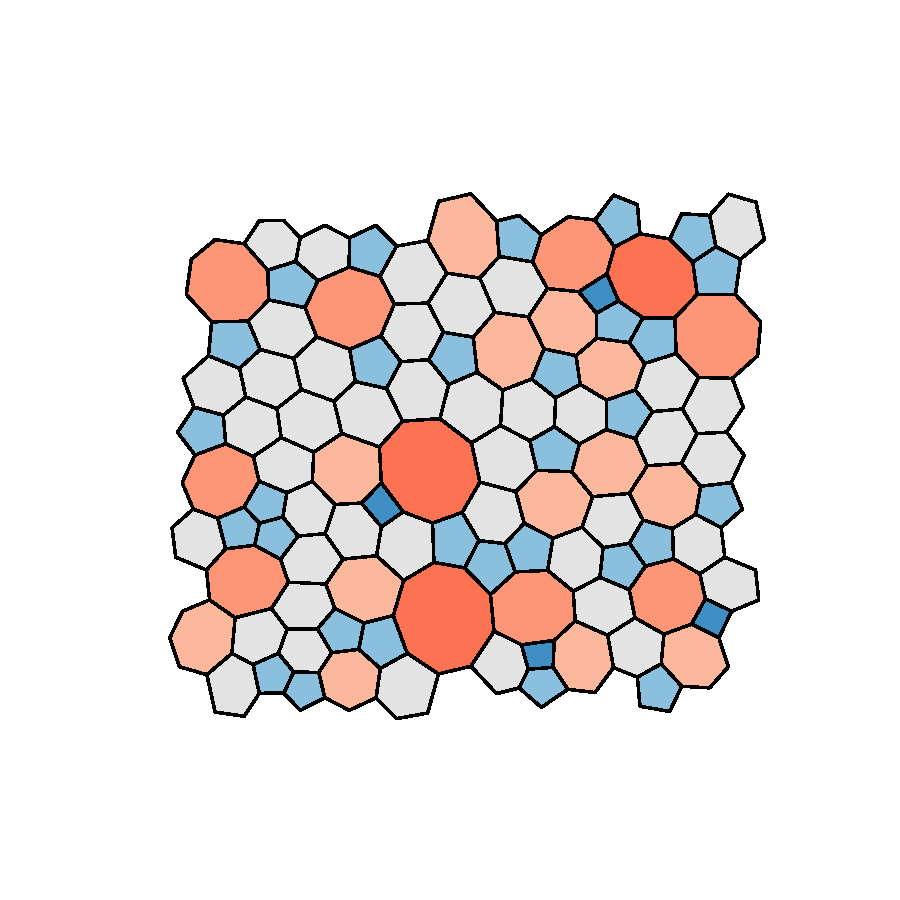
\includegraphics[height=4cm]{./figures/general_networks/silica.pdf}
         \caption{Planar, $c=3$, \\ length controlled.}
         \label{fig:ne1}
     \end{subfigure}
     \hfill
     \begin{subfigure}[b]{0.25\textwidth}
         \centering
         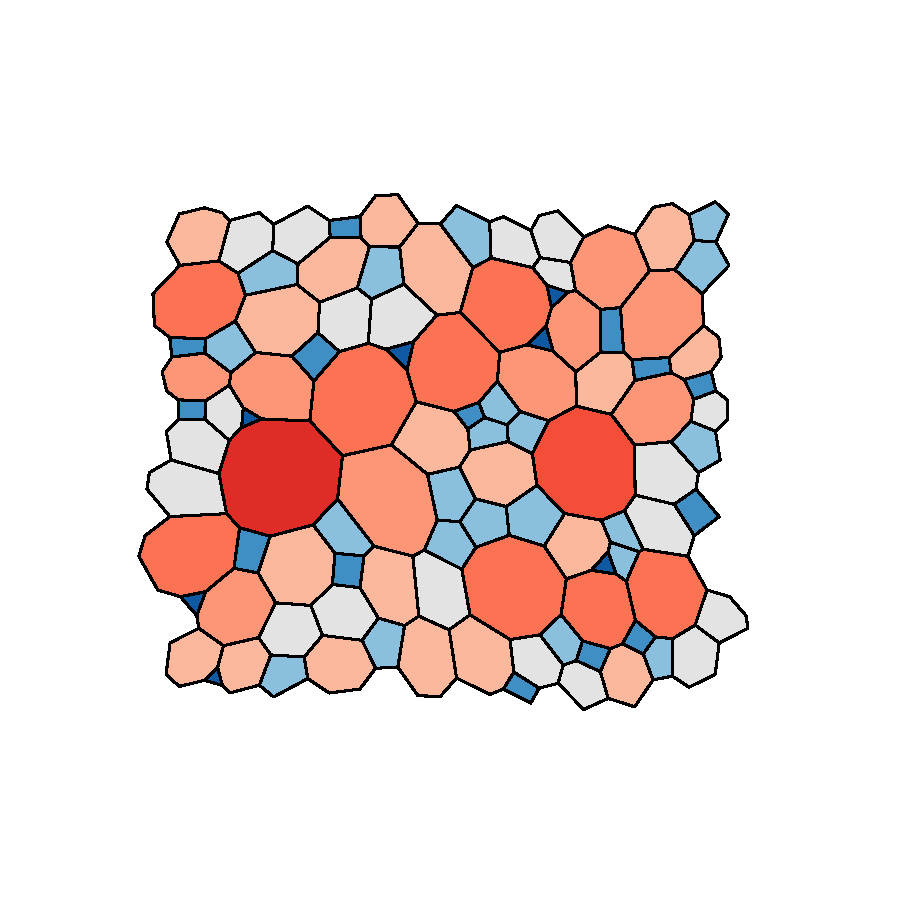
\includegraphics[height=4cm]{./figures/general_networks/foam.pdf}
         \caption{Planer, $c=4$, \\ angle controlled.}
         \label{fig:ne2}
     \end{subfigure}
     \hfill
     \begin{subfigure}[b]{0.25\textwidth}
         \centering
         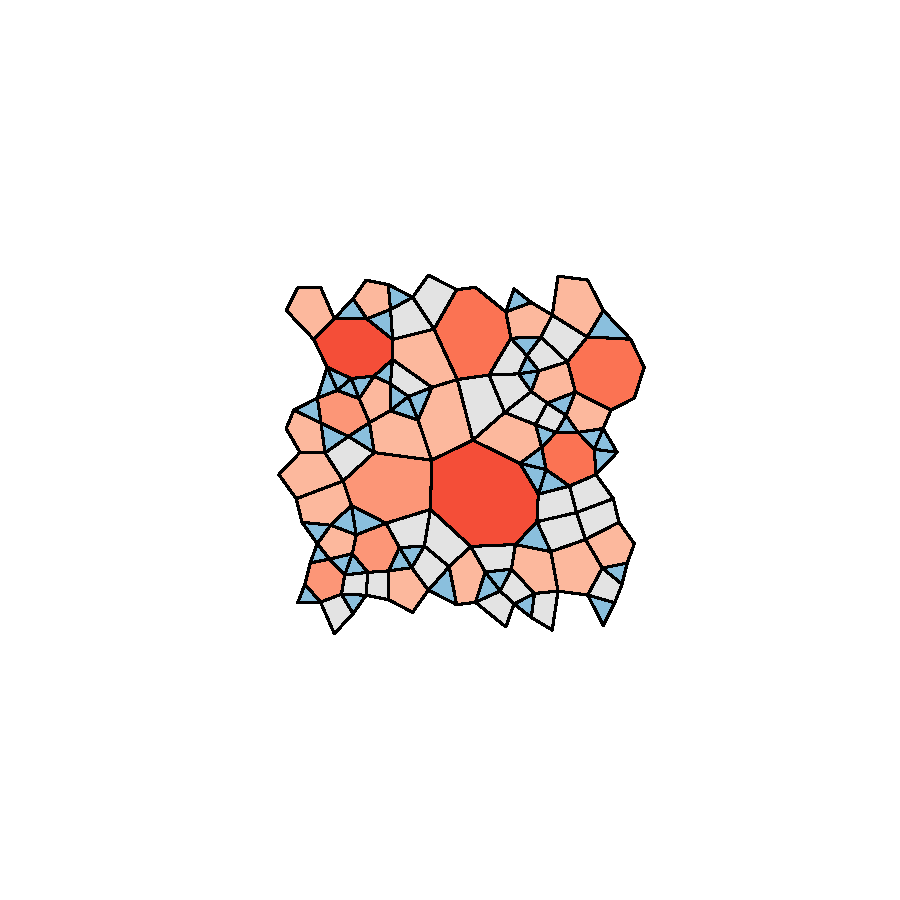
\includegraphics[height=4cm]{./figures/general_networks/four.pdf}
         \caption{Planer, $c=4$, \\ angle controlled.}
         \label{fig:ne3}
     \end{subfigure}
     \hfill
     
     \vspace{0.2cm}
      \begin{subfigure}[b]{0.25\textwidth}
         \centering
         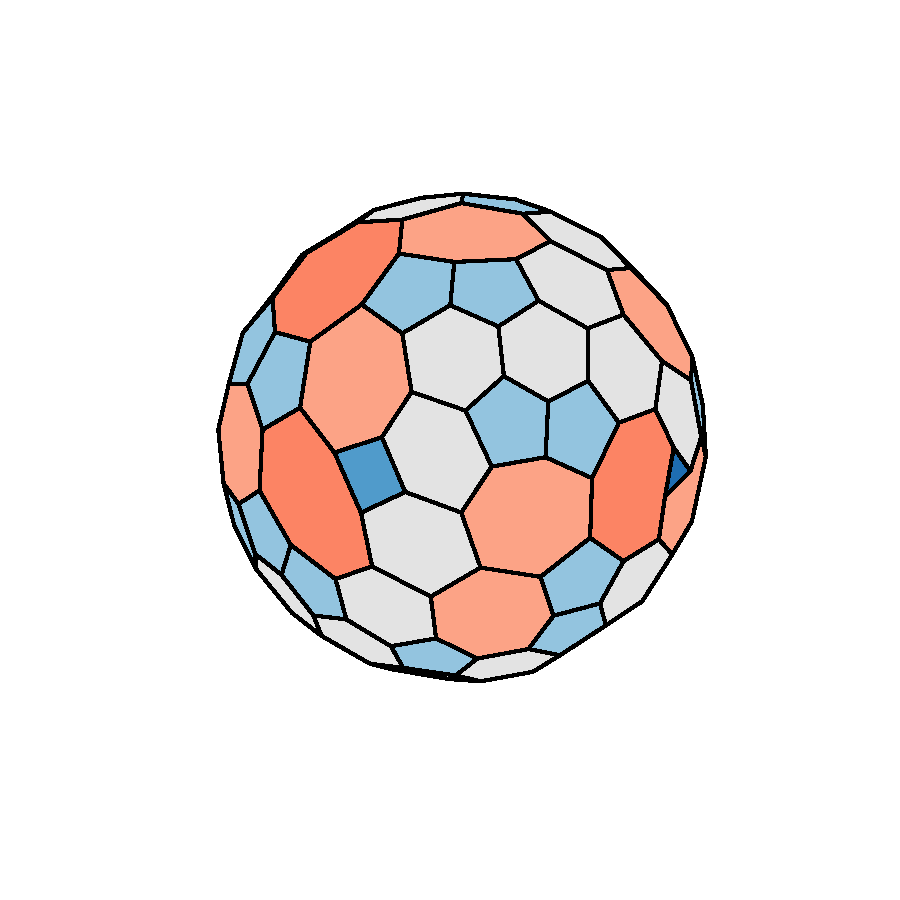
\includegraphics[height=4cm]{./figures/general_networks/afull92.pdf}
         \caption{Spherical, $c=3$.}
         \label{fig:ne4}
     \end{subfigure}
     \hfill
     \begin{subfigure}[b]{0.25\textwidth}
         \centering
         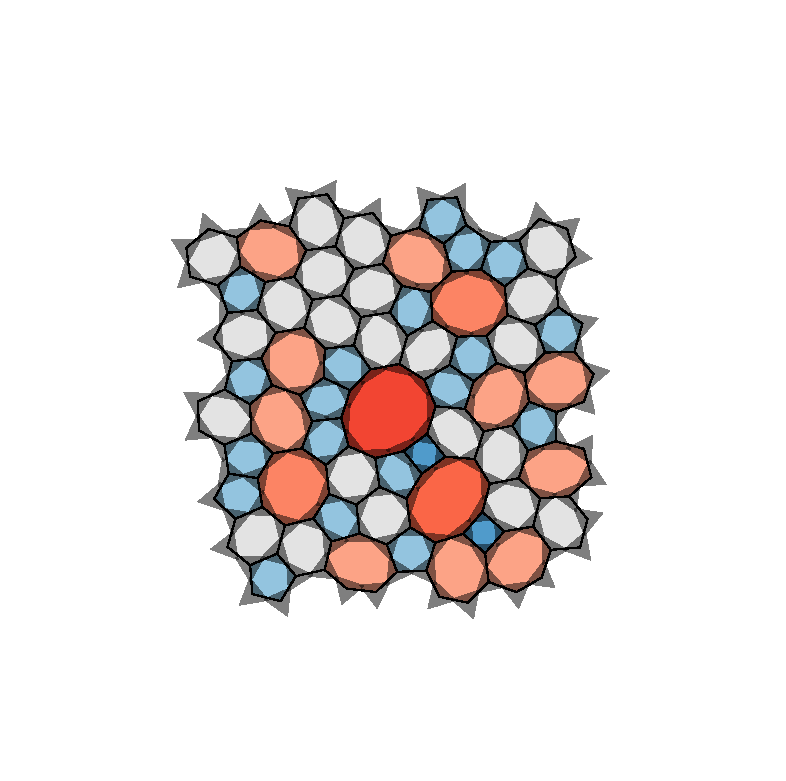
\includegraphics[height=4cm]{./figures/general_networks/traft.pdf}
         \caption{Triangle raft.}
         \label{fig:ne5}
     \end{subfigure}
     \hfill
     \begin{subfigure}[b]{0.25\textwidth}
         \centering
         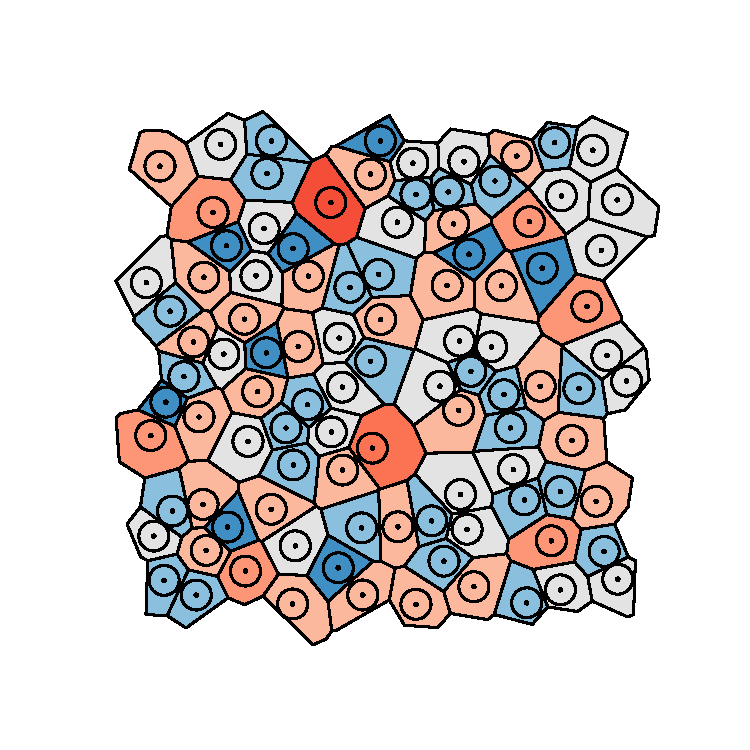
\includegraphics[height=4cm]{./figures/general_networks/colloid.pdf}
         \caption{Hard disk Voronoi.}
         \label{fig:ne6}
     \end{subfigure}
     \hfill
     
     \vspace{0.2cm}
     \begin{subfigure}[b]{0.5\textwidth}
         \centering
         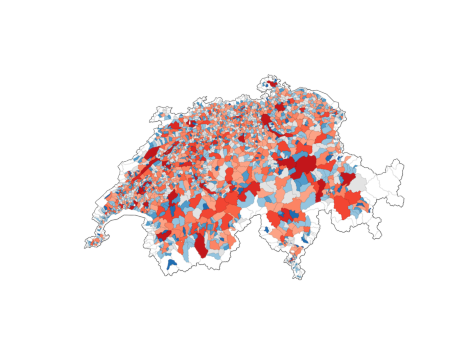
\includegraphics[width=\textwidth]{./figures/general_networks/ch_lowres.pdf}
         \caption{Communes of Switzerland.}
         \label{fig:ne7}
     \end{subfigure}

     \caption{Two-dimensional networks emerge in diverse physical systems and span a range of length scales, coordination environments,
and topologies: (a) 3-coordinate, bond\--length controlled network, \eg, glass; (b) 3\--coordinate, angle controlled network, \eg{} foam; (c) 4\--coordinate network; (d) 3\--coordinate network in spherical geometry, \eg{} nonclassical fullerene; (e) triangle raft, \eg{} silica bilayer; (f) hard disk Voronoi \eg{} colloidal monolayer; and (g) communes of Switzerland. Rings are coloured similarly according to size with blue, gray, and red indicating smaller than, equal to, and greater than the mean ring size, respectively.}
     \label{fig:networkexamples}
\end{figure}

\section{Generalised Network Theory}

A consequence of the universality of \td{} networks is that both the language and the metrics used to describe then varies considerably between fields, as demonstrated in table \ref{tab:genterms}.
From a nano\--materials perspective there are rings formed from a set of bonded atoms, in crystals there are grains separated by boundaries and in biological tissues cells which divide.
Further complication may arise from the concept of graph duality, where ring structure emerges only after transforming the physical coordinates.
In the context of colloidal monolayers for instance, rings are generated using the Voronoi construction; where the vertices have no real manifestation and the particle positions are the simplices in the dual Delaunay triangulation.
In addition as seen in previous chapters, there remains a prevalence of empirical laws to describe their structure.

\begin{table}[bt]
	\centering
     \caption{Terminology to describe ring structure in literature reflects the diversity of the underlying physical systems.}
     \label{tab:genterms}
     \begin{tabular}{cc}
     \toprule
     Term & Synonyms and Examples \\
     \midrule
     Ring & Face, polygon, cell, grain, pore, Voronoi cell\\
     Network & Graph, tiling, packing, tessellation, partition, \\
     & arrangement, decomposition, net, mosaic\\
     Link & Edge, bond, boundary, interface \\
     Node & Vertex, point, atom \\
     \bottomrule
     \end{tabular}
\end{table}
Network science offers an opportunity to unite the study of these disparate physical systems through a generalised theory.
Much of the groundwork for this has been laid in chapter \ref{ch:networktheory}, but there are some important additions, namely the introduction of the assortativity to describe ring\--ring correlations.
Some of the key aspects which were introduced in chapter \ref{ch:networktheory} will be briefly recapped, before these extensions are highlighted.

Chapters \ref{ch:targetedopt} and \ref{ch:bilayers} of this thesis focussed on planar atomic systems which had a fixed coordination of three.
The main difference in this chapter is that the scope has increased to include networks with variable coordination and topologies.
For generic physical networks the equivalent of the atomic coordination number, $c$, is not necessarily precisely defined by an atomic species. 
The consequence of this is that the mean ring size as dictated by Euler's law is no longer always six, but rather determined by equations \eqref{eq:2dplanarcases},\eqref{eq:2dsphericalcases}; so that for example a network of $c=4$ will have a mean ring size of $\ki=4$.
That being said, the majority of naturally occurring networks still have $c=3$, as higher order sites are unstable with respect to small perturbations, with for example a 4\--coordinate site readily splitting into two 3\--coordinate sites \cite{Caer1993}.

The ring statistics, $p_k$, remain an important measure, and have a clear analogue in network science, being the node degree distribution of the ring network (see section \ref{s:atomringnetworks}).
The node degree distribution is still expected to follow \lm's maximum entropy distribution, provided the constraints are appropriately adjusted to reflect the mean node degree.
Whilst all natural networks lie on the universal \lm{} curve, it will be seen in section \ref{s:gendegreedist}, that the specific location of a given network is dependent on the underlying physics of the system.

The other empirical law heavily discussed in this thesis, the \aw{} law, is more problematic.
Although it has proved useful in materials science, it is largely confined to this area, and is not without flaws.
These flaws will be discussed in detail below, but they essentially arise from the empiricism of the law and the resulting difficulty in interpreting its results.
However, network science has a well\--adopted metric for measuring node degree correlations, termed the assortativity.  
This chapter therefore provides a good opportunity to replace the empirical \aw{} law with a concrete measure, and it will be shown in section \ref{s:assortativity} that there is a mapping between the \aw{} parameter and the assortativity.

\subsection{Deficiencies in the Aboav\--Weaire Law}

For all its perceived success in characterising amorphous materials, the \aw{} law suffers from several deficiencies, some of them academic and others practical.
To begin with, it remains the case that despite numerous efforts \cite{Lambert1981,Kumar1994,Blanc1979,Rivier1985,Peshkin1991,Chiu1994} there is no satisfactory theoretical justification behind the \aw{} law; the various attempts and their drawbacks summarised excellently by Mason \etal{} \cite{Mason2012}.
In fact it seems increasingly likely that the difficulty in finding an adequate theoretical proof for the \aw{} law simply arises from the fact that there just isn't a strong physical basis behind it.

One may then reasonably question why the linear \aw{} law holds so well for a range of different systems.
The answer again may be the fact that unfortunately it is not as infallible as its widespread usage would suggest.
In particular the assumption that the law holds and is indeed linear is often overlooked.
This is not in reference to somewhat contrived examples, such as regular crystalline arrangements, as the \aw{} law is a really a comment on disordered systems \cite{Boots1984}.
Even ``conventional'' examples often show deviations \cite{Earnshaw1994,Kumar1994,Hilhorst2006}.
These manifest in two ways.
Firstly the data may not be linear over the whole range.
This size of this effect can be understated, as such deviations from linearity occur in the tails of the ring distribution at low or high $k$, where the discrepancy is often attributed to poor sampling statistics.
Nevertheless, as Mason \etal{} astutely point out \textit{``a linear model is a good approximation of any smooth function over a small domain, and that the success of the law of \aw{} does not necessarily indicate that the average excess curvature is actually linear''}.
The second issue is that little attention is paid to the exact form of the law and the fact that the intercept should be $\ki^2+\mu_2$ is rarely adhered to.
Enforcing this condition often leads to a less satisfactory fit. 

The consequences of the difficulty in obtaining an accurate \aw{} fit are naturally that the resulting $\alpha$ parameter has associated with it a degree of ``greyness''.
Yet even in the case where the \aw{} law seems wholly appropriate, there is still a difficulty in fully interpreting its meaning.
It is not intuitive what the actual value of $\alpha$ represents nor its limits.
Even for a simple system of $\left\{5,6,7\right\}$ rings, equation \eqref{eq:agalpha} illustrated that the relationship between ring structure and $\alpha$ is non\--trivial.
More generally, it was shown in section \ref{s:awlaw}, if rings are arranged purely randomly that $\alpha=-\frac{\mu_2}{\ki^2}$, but without a well\--defined upper limit for comparison interpretation remains restricted.
This equation also highlights that $\alpha$ is dependent on the ring statistics and that its sign is an insufficient classifier for positive or negative correlation.
Hence even if a high quality fit is achieved, a combination of these effects make it difficult to draw accurate comparisons between different systems.

This is not to say that the \aw{} law does not have value, and certainly the general observation is extremely interesting, even if the underlying relationship is more complex than originally suggested.
It is more to point out that there is scope to improve the quantification of the effect and that a robust approach which is applicable to diverse systems will be required to study generic \td{} networks.

\subsection{Assortativity as a Measure of Ring Size Correlations}
\label{s:assortativity}

The assortativity was introduced by Newman to measure the preference of low degree nodes to be adjacent to high degree nodes in generic networks \cite{Newman2002}.
It has proved highly popular in the network science and the study of social and biological networks \cite{Noldus2015}, but has also been applied for example in theoretical studies of hard disk packings \cite{Chremos2007}.
The calculation of the assortativity revolves around the edge joint degree distribution, $e_{jk}$, which measures the probability of two nodes of degrees $j$,$k$ sharing a link (\ie{} two rings of sizes $j$,$k$ being adjacent).
The probability of any link having degree $k$ is distributed according to $q_k=kp_k/\ki$, and so if nodes are randomly arranged $e_{jk}=q_j q_k$.
Deviation from this random arrangement is the assortativity, and can be measured by Pearson's correlation coefficient:
\begin{equation}
        \label{eq:assortativity}
        r = \frac{\sumjk jk\left(e_{jk}-q_jq_k\right)}{\sumk k^2q_k - \left(\sumk kq_k\right)^2}=\frac{\ki^2\sumjk jke_{jk}-\kii^2}{\ki\kiii-\kii^2}\,.
\end{equation}
For this coefficient to be calculable, the second and third moments of the degree distribution must be finite \cite{Litvak2013}.
This condition is satisfied for these physical systems, as the proportion of large rings quickly becomes vanishingly small.

\begin{figure}[bt]
     \centering
       
     \begin{subfigure}[b]{0.32\textwidth}
         \centering
         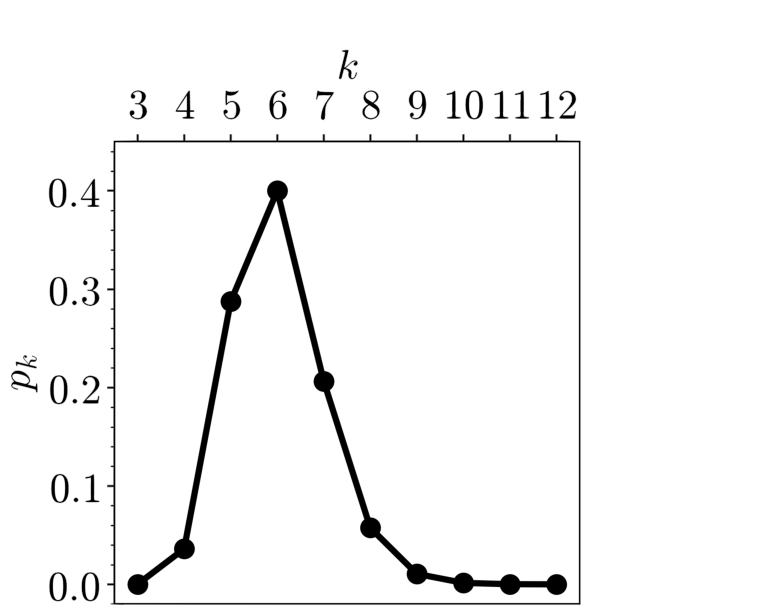
\includegraphics[width=\textwidth]{./figures/general_networks/assort_mat_pk.pdf}
         \caption{$p_k$}
         \label{fig:rexa}
     \end{subfigure}
     \hfill
     \begin{subfigure}[b]{0.205\textwidth}
         \centering
         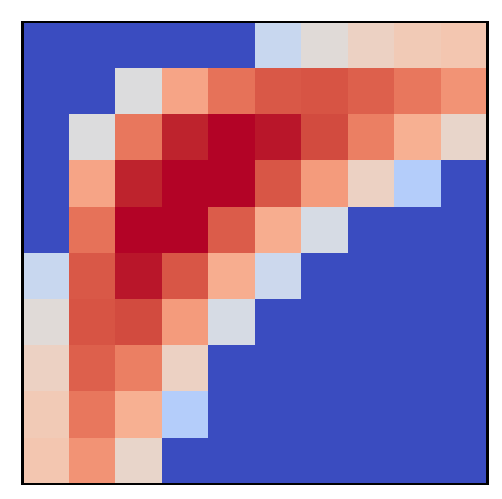
\includegraphics[width=\textwidth]{./figures/general_networks/assort_mat_-75.pdf}
         \caption{$r=-0.75$}
         \label{fig:rexb}
     \end{subfigure}
     \hfill
     \begin{subfigure}[b]{0.205\textwidth}
         \centering
         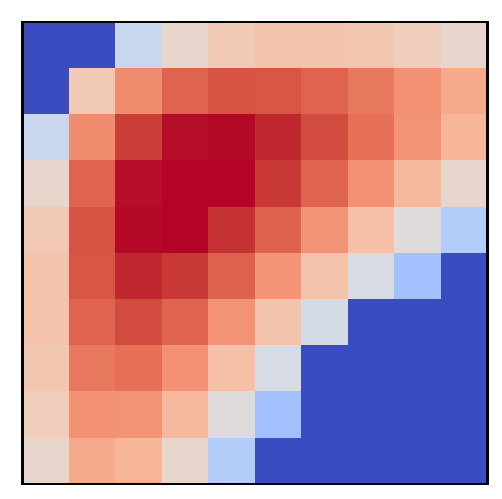
\includegraphics[width=\textwidth]{./figures/general_networks/assort_mat_-50.pdf}
         \caption{$r=-0.50$}
         \label{fig:rexc}
     \end{subfigure}
     \hfill
     \begin{subfigure}[b]{0.205\textwidth}
         \centering
         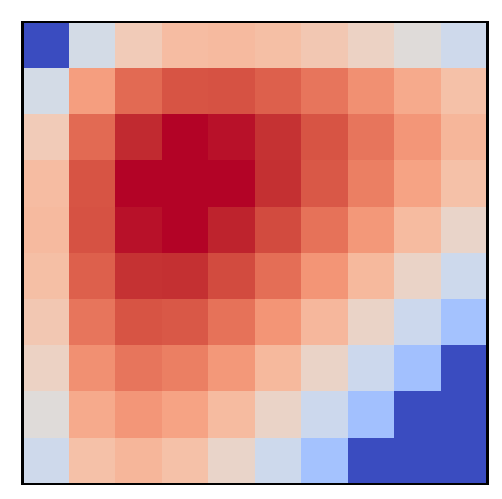
\includegraphics[width=\textwidth]{./figures/general_networks/assort_mat_-25.pdf}
         \caption{$r=-0.25$}
         \label{fig:rexd}
     \end{subfigure}
     \hfill
     
        \begin{subfigure}[b]{0.32\textwidth}
         \centering
         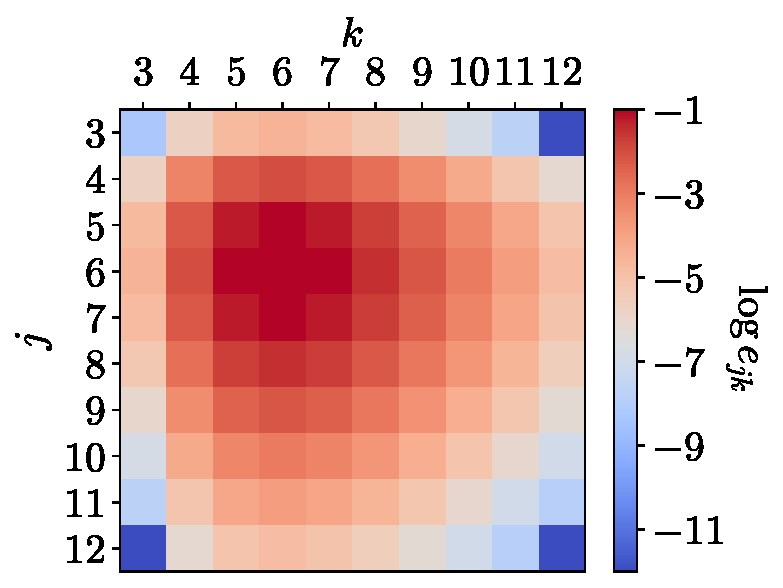
\includegraphics[width=\textwidth]{./figures/general_networks/assort_mat_0.pdf}
         \caption{$r=0.00$}
         \label{fig:rexe}
     \end{subfigure}
     \hfill
     \begin{subfigure}[b]{0.205\textwidth}
         \centering
         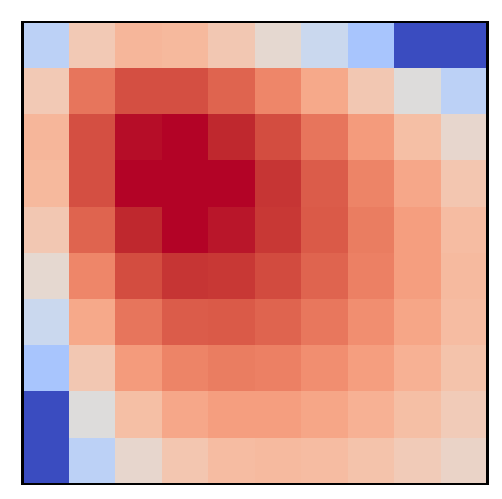
\includegraphics[width=\textwidth]{./figures/general_networks/assort_mat_25.pdf}
         \caption{$r=0.25$}
         \label{fig:rexf}
     \end{subfigure}
     \hfill
     \begin{subfigure}[b]{0.205\textwidth}
         \centering
         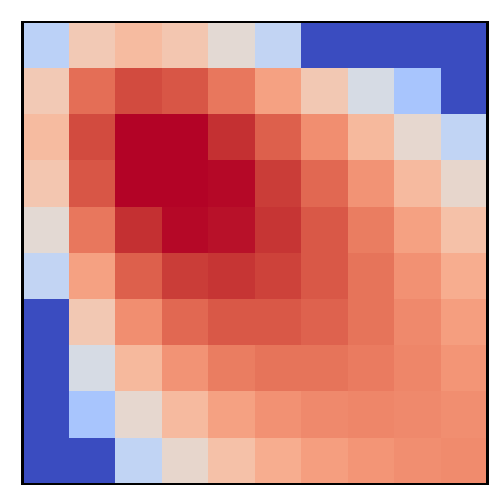
\includegraphics[width=\textwidth]{./figures/general_networks/assort_mat_50.pdf}
         \caption{$r=0.50$}
         \label{fig:rexg}
     \end{subfigure}
      \hfill
       \begin{subfigure}[b]{0.205\textwidth}
         \centering
         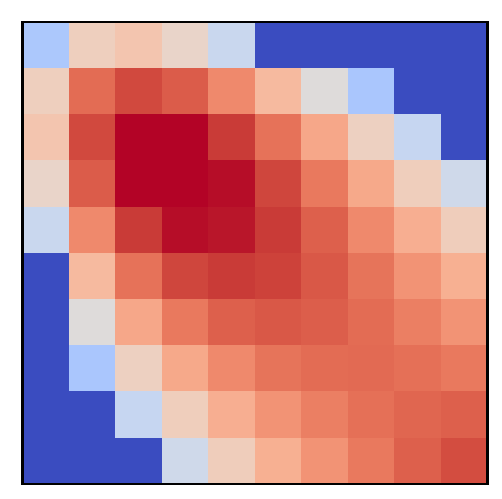
\includegraphics[width=\textwidth]{./figures/general_networks/assort_mat_75.pdf}
         \caption{$r=0.75$}
         \label{fig:rexh}
     \end{subfigure}
      \hfill
 
     \caption{Visualisation of the joint node degree distribution, $e_jk$, for a given node degree distribution, $p_k$, at different assortativities, $r$. Panel (a) gives the node degree distribution (\ie{} ring statistics), and panels (b)\--(h) visualisations of the joint node degree distribution at increasing assortativities. All matrices have the same orientation and colouring as panel (e).}
     \label{fig:rex}
\end{figure}

The advantages of adopting this measure of assortativity are clear.
The correlation coefficient is bounded between $-1\leq r \leq 1$ and has three well defined limits: $r=0$ indicating a random network, $r=1$ a perfectly assortative network and $r=-1$ a perfectly disassortative network.
Intermediate values of $r$ are then readily understandable in reference to these limits, with a concomitant effect on the joint degree distribution, as illustrated in figure \ref{fig:rex}. 
This allows physical networks to be readily compared in a way that the \aw{} law does not allow.
Physical networks can now be fitted in to the wider field of network science, introducing them as important examples alongside more traditionally studied networks.
Using the assortativity also provides a natural extension to higher dimensions, which has been difficult to reconcile with the empirical \aw{} law \cite{Mason2012}.

For completeness, it will be shown that the assortativity can be related to the \aw{} parameter.
This can be achieved by using the fact that that the mean node degree about a $j$-degree node is given in equation \eqref{eq:mjejklink} as $q_jm_j=\sumk ke_{jk}$.
Substituting this expression into equation \eqref{eq:assortativity}, and assuming the \aw{} law \eqref{eq:aboavweaire} holds \textit{exactly}, it can be shown that:
\begin{equation}
        \label{eq:rawlink}
        \alpha = - \frac{r\left(\ki\kiii-\kii^2\right)}{\mu_2\ki^2}-\frac{\mu_2}{\ki^2},
\end{equation}
which is consistent with the topological gas, when $r=0$.
The derivation of this result is given in appendix \ref{app:derivalphaassort}.
In reality, the \aw{} fit is never perfect, and so equation \eqref{eq:rawlink} provides an approximation to the value of $\alpha$. 
The accuracy of this equation will therefore depend on the applicability of the linear fit.
\davidnote{Include that figure somewhere}.

The assortativity also provides a natural framework to extend \lm's maximum entropy arguments to factor in ring adjacencies.
The entropy is first defined in terms of the edge joint degree distribution, as $S=-\sumjk e_{jk}\log e_{jk}$.
Considering $e_{jk}$, the following constraints must hold:
\begin{align}
        \sumjk e_{jk} &=1 \label{con:as1}\\
        \sumjk ke_{jk} &= \frac{\mu_2}{\ki}+\ki \label{con:as2}\\
        \sumjk \frac{1}{j}e_{jk} &= \frac{1}{\ki} \label{con:as3}\\
        \sumjk jke_{jk} &= c\left(r\right)\label{con:as4};
\end{align}
resulting from the normalisation condition, Weaire's sum rule \cite{Weaire1974} and Euler's formula and finally a constraint imposing the assortativity from equation \eqref{eq:assortativity}.
As for \lm's law, Lagrange's method can be used with the constraints above (noting that $e_{jk}=e_{kj}$) to generate a maximum entropy joint distribution which satisfies:
\begin{equation}
        \label{eq:mer}
        e_{jk} = \frac{e^{-\frac{\lambda_1}{2}\left(j+k\right)-\frac{\lambda_2}{2}\left(1/j+1/k\right)-\lambda_3 jk}}{\sumjk e^{-\frac{\lambda_1}{2}\left(j+k\right)-\frac{\lambda_2}{2}\left(1/j+1/k\right)-\lambda_3 jk}},
\end{equation}
and equations \eqref{con:as2}\--\eqref{con:as4}.
This can again be solved numerically, and the resulting distribution can be related to a single node degree probability (\eg{} $p_6$) and an assortativity value.

\section{Generalised Bond Switching Algorithm}
\label{s:genbondswitching}

In order to study generic physical networks, a simulation method is required which can generate configurations across a wide range of coordination environments, topologies and potential models. 
The bond switching algorithm, introduced in section \ref{s:bondswitch}, is a good candidate as it has proved effective for studying atomic networks in chapter \ref{ch:targetedopt}.
However, currently it is only adapted to study constant coordination planar systems (in this work 3\--coordinate but there is one previous example of study of 4\--coordinate systems \cite{Greneche1990}).
Therefore a further natural extension of the bond switching method is presented here, to variable atomic coordination environments and overall system topology.

As a review from a networks perspective, the bond switching algorithm is a stochastic sampling method.
Starting from an initially well\--ordered network, links between neighbouring nodes are switched and the effect on the potential energy of the system (\ie{} the amount of strain which is introduced or removed) is calculated.
The energy of the system is determined by the potential model, which expresses the total energy of the network as a function of all node positions.
After the links between nodes are switched, geometry optimisation of the node positions takes place to minimise the total potential energy.
By incorporating switches which reduce the potential energy of the network with greater probability, one can bias the search towards networks of lower energy and therefore which occur more commonly in nature.
The specificities of the algorithm will however depend on the exact nature of the system in question.

\subsection{Extension to Variable Coordination}

The choice of the starting lattice can be used to determine the system properties \ie{} the atomic coordination environments and topologies (table \ref{tab:lattices}, figure \ref{fig:lattices}).
This is because in the bond switching algorithm the node degree distribution of the atomic network is constant, and hence from equation \eqref{eq:avdegree} so is mean node degree of the dual network.
Therefore whichever topology, atomic coordinations and mean ring size the system is initialised with will be preserved throughout the simulation.

\begin{table}
   \centering
     \caption{List of starting crystalline lattices for bond switching for a range of coordination environments, and the corresponding mean ring size.}
     \label{tab:lattices}
     \begin{tabular}{ccccc}
     \toprule
     Topology & $x_3$ & $x_4$ & $\ki$ & Lattice\\
     \midrule
        Planar & $1$ & $0$ & $6$ & Hexagonal \\
        Planar & $0$ & $1$ & $4$ & Square \\
        Planar & $2/3$ & $1/3$ & $5$ & Cairo \\
        Planar & $x_3$ & $x_4$ & $4\rightarrow6$ & Mixed Hexagonal\--Square \\
        Spherical & $1$ & $0$ & $\sim 6$ & $12$-Pentagon Fullerene \\
        Spherical & $0$ & $1$ & $\sim 4$ & $8$-Triangle Fullerene \\
        \bottomrule
     \end{tabular}
\end{table}

The bond switching move will then vary depending on the coordination properties, as outlined in figure \ref{fig:bsmoves}.
Figures \ref{fig:bsmovea}\--\ref{fig:bsmovec} show the original move, which was designed for purely 3\--coordinate atoms, and is in effect introducing a Stone\--Wales defect.
This move augments the ring size of two rings and decrements two others, preserving both the mean ring size and the coordination number of the individual atoms involved in the transformation.
The changes in ring size (equivalent to the changes in node degree of the dual network) are highlighted in the figure as ``$\pm{1}$''.
The extension to 4\--coordinate atoms (figures \ref{fig:bsmoved}\--\ref{fig:bsmovef}) is relatively straightforward, simply involving extra spectator atoms, but for mixed coordination it is subtly different (figures \ref{fig:bsmoveg}\--\ref{fig:bsmovei}).
For the both systems the local ring sizes are again changed by $\pm{1}$ (as highlighted, and preserving the mean ring size).
However, whereas for the pure systems the switch move must be coordination preserving, for mixed coordination systems this prevents true melting.
This can be countered by using a move in which the coordinations of neighbouring atoms are exchanged, whilst maintaining a constant mean ring size.

\begin{figure}[bt]
     \centering
     
     \begin{subfigure}[b]{0.25\textwidth}
         \centering
         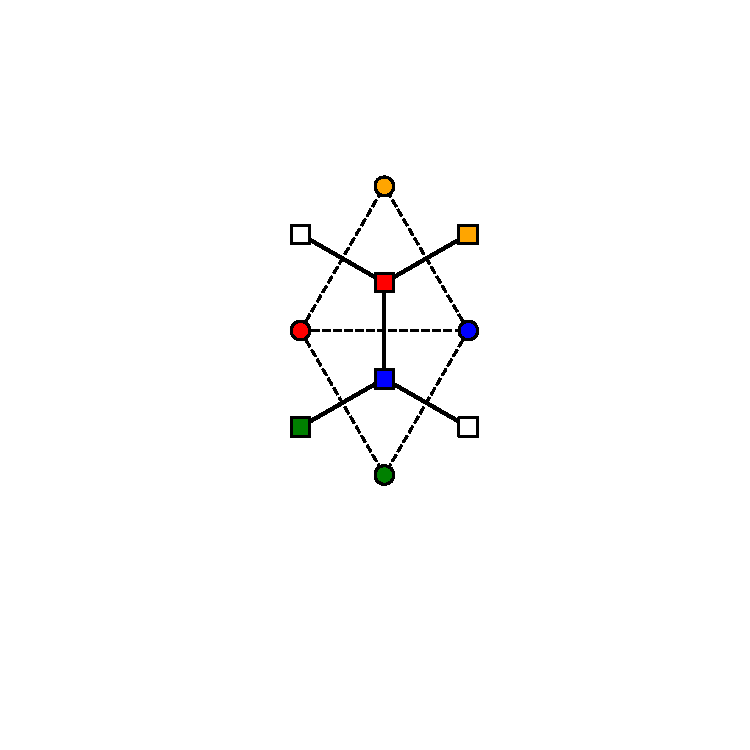
\includegraphics[height=2.6cm]{./figures/general_networks/bs_move_a.pdf}
         \caption{Initial $c=3$.}
         \label{fig:bsmovea}
     \end{subfigure}
     %{\LARGE$\rightarrow$}
     \hfill
     \begin{subfigure}[b]{0.25\textwidth}
         \centering
         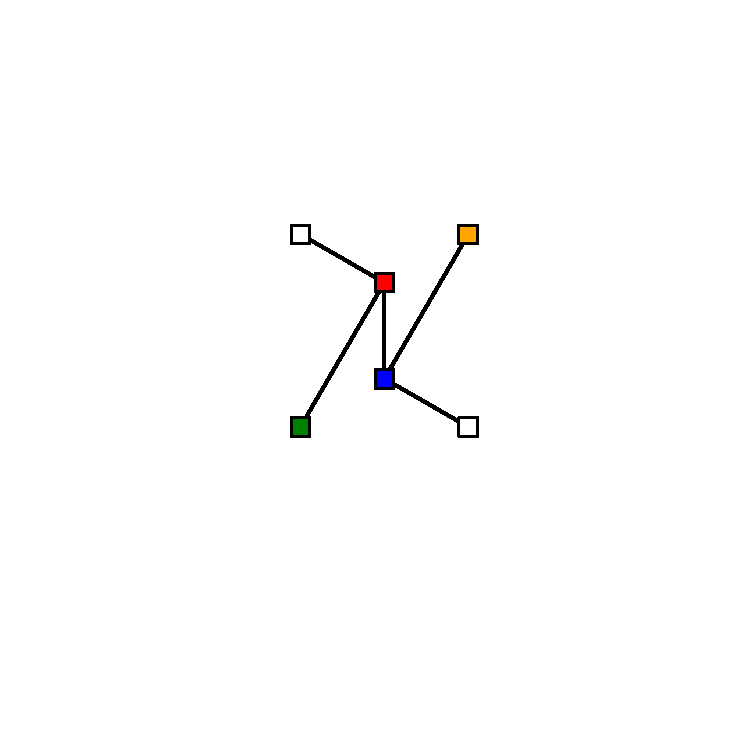
\includegraphics[height=1.8cm]{./figures/general_networks/bs_move_b.pdf}
         \caption{Switched $c=3$.}
         \label{fig:bsmoveb}
     \end{subfigure}
     %{\LARGE$\rightarrow$}
     \hfill
     \begin{subfigure}[b]{0.25\textwidth}
         \centering
         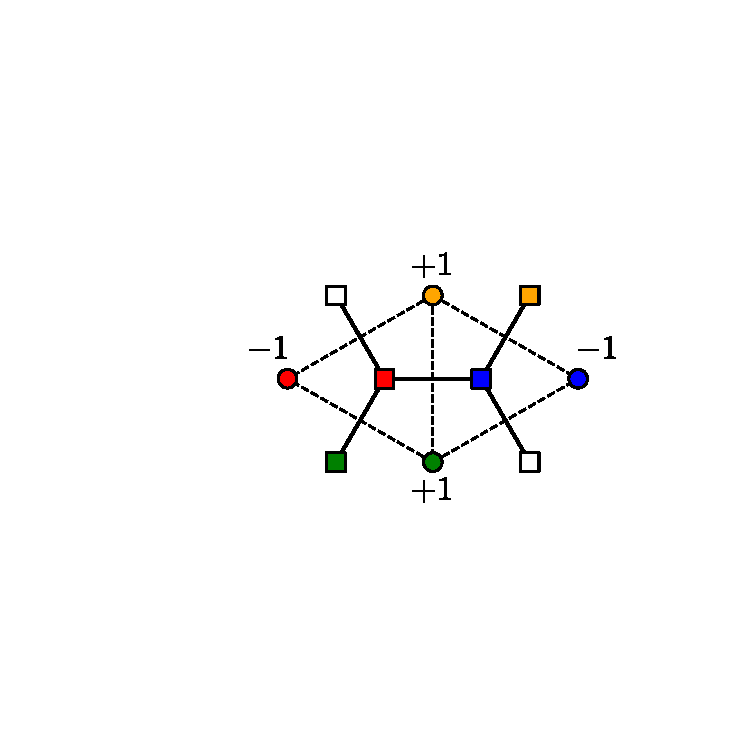
\includegraphics[height=2.1cm]{./figures/general_networks/bs_move_c.pdf}
         \caption{Optimised $c=3$.}
         \label{fig:bsmovec}
     \end{subfigure}
     
     \vspace{5mm}
     \begin{subfigure}[b]{0.25\textwidth}
         \centering
         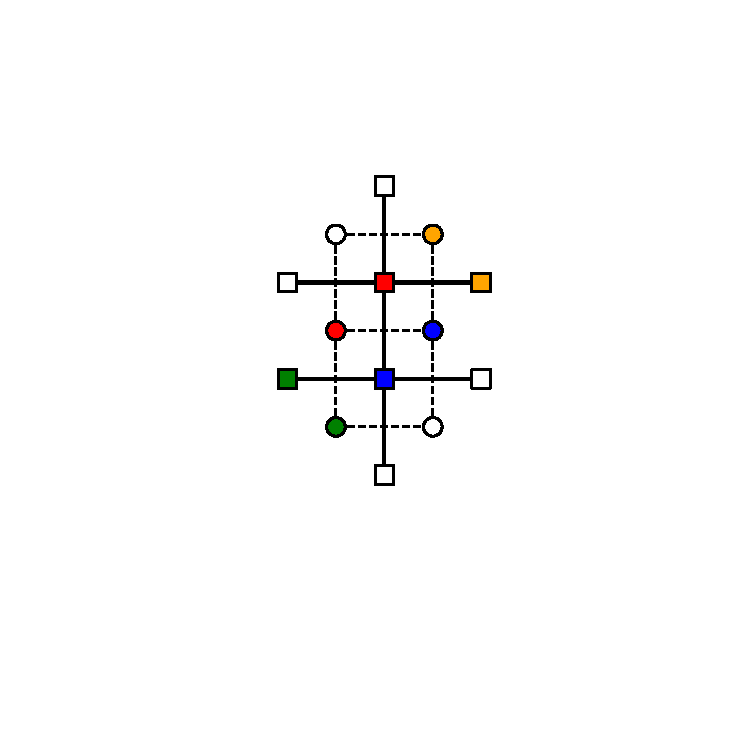
\includegraphics[height=2.6cm]{./figures/general_networks/bs_move_d.pdf}
         \caption{Initial $c=4$.}
         \label{fig:bsmoved}
     \end{subfigure}
     %{\LARGE$\rightarrow$}
     \hfill
     \begin{subfigure}[b]{0.25\textwidth}
         \centering
         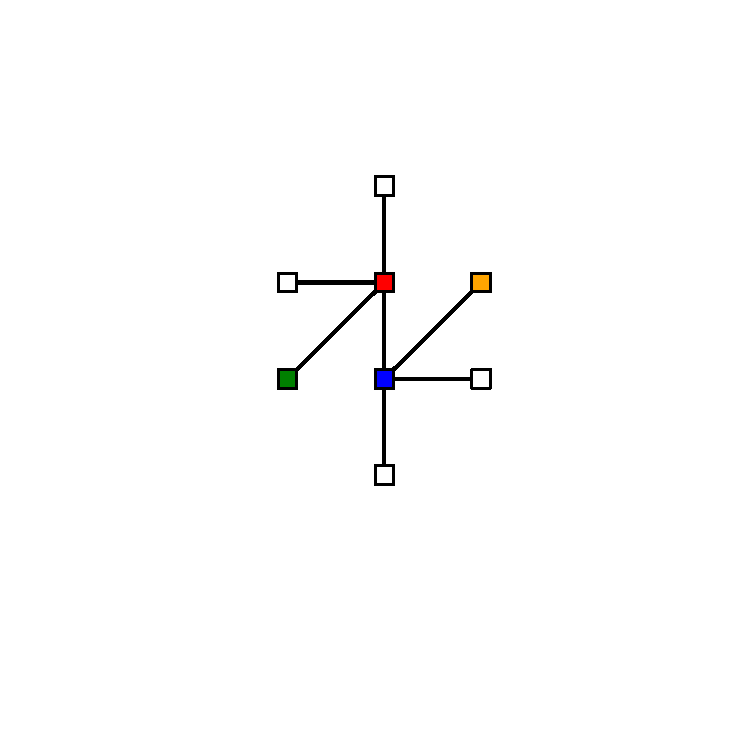
\includegraphics[height=2.6cm]{./figures/general_networks/bs_move_e.pdf}
         \caption{Switched $c=4$.}
         \label{fig:bsmovee}
     \end{subfigure}
     %{\LARGE$\rightarrow$}
     \hfill
     \begin{subfigure}[b]{0.25\textwidth}
         \centering
         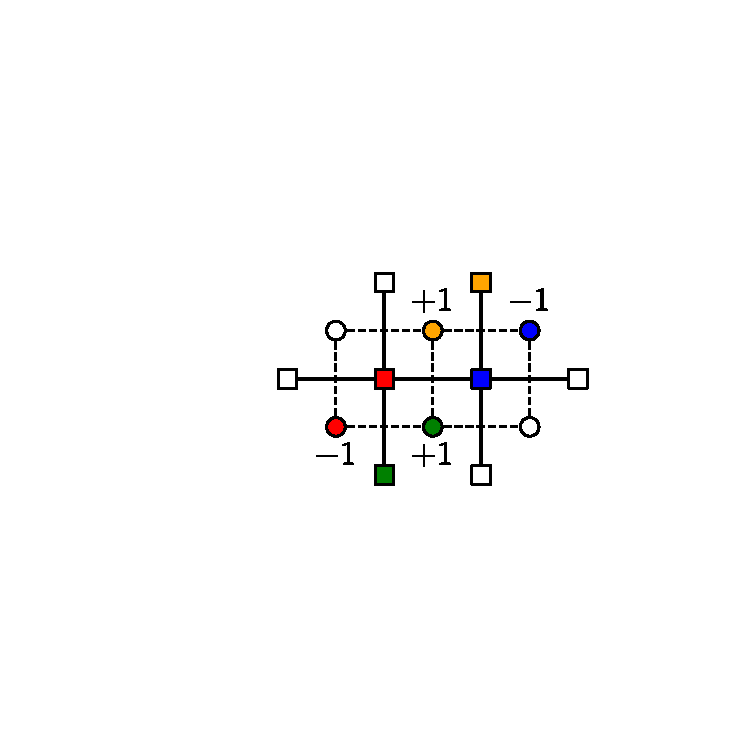
\includegraphics[height=1.8cm]{./figures/general_networks/bs_move_f.pdf}
         \caption{Optimised $c=4$.}
         \label{fig:bsmovef}
     \end{subfigure}
     
     \vspace{5mm}
     \begin{subfigure}[b]{0.25\textwidth}
         \centering
         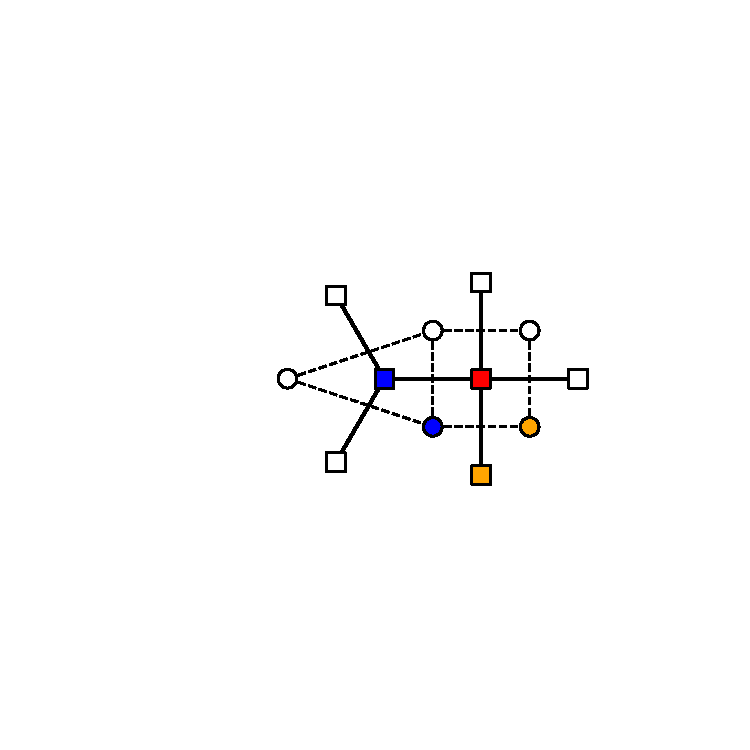
\includegraphics[height=1.8cm]{./figures/general_networks/bs_move_g.pdf}
         \caption{Initial $c=3,4$.}
         \label{fig:bsmoveg}
     \end{subfigure}
     %{\LARGE$\rightarrow$}
     \hfill
     \begin{subfigure}[b]{0.25\textwidth}
         \centering
         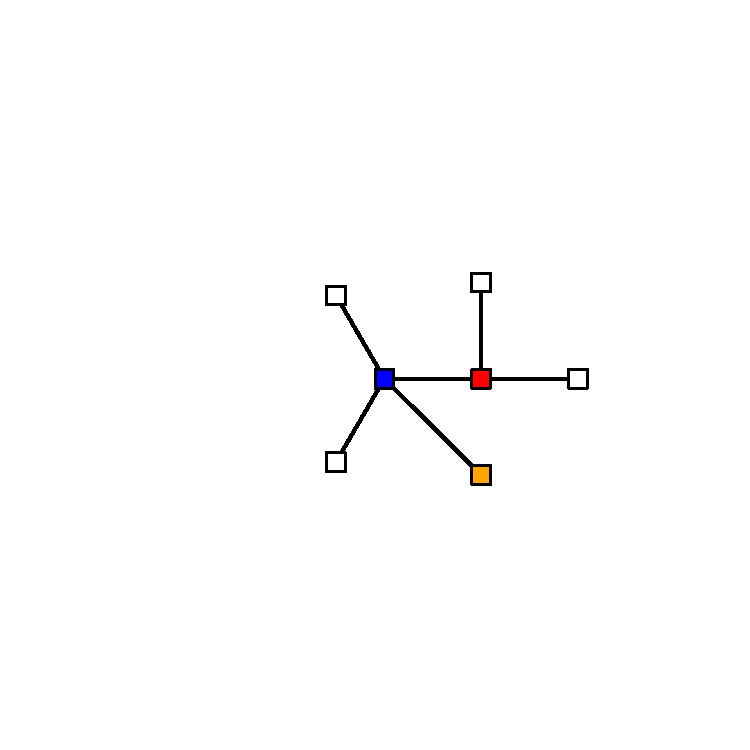
\includegraphics[height=1.8cm]{./figures/general_networks/bs_move_h.pdf}
         \caption{Switched $c=4,3$.}
         \label{fig:bsmoveh}
     \end{subfigure}
     %{\LARGE$\rightarrow$}
     \hfill
     \begin{subfigure}[b]{0.25\textwidth}
         \centering
         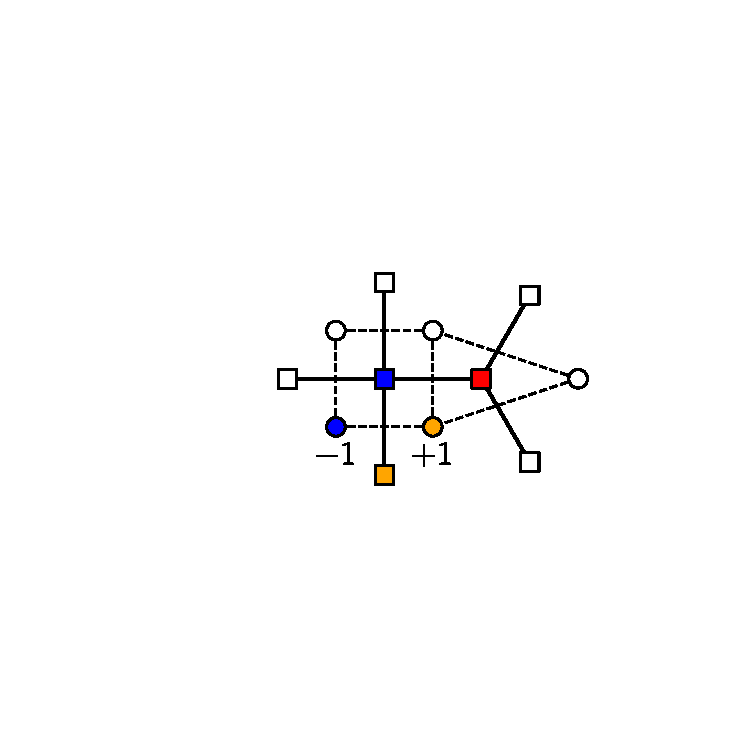
\includegraphics[height=1.8cm]{./figures/general_networks/bs_move_i.pdf}
         \caption{Optimised $c=4,3$.}
         \label{fig:bsmovei}
     \end{subfigure}
     
     \caption{Bond switching Monte Carlo moves for different atomic coordination environments: 3\--coordinate sites (a)-(c), 4\--coordinate sites (d)-(f) and mixed 3/4 coordination (g)-(i). For each coordination type the atomic connectivity is shown for the starting structure (left), the initial switched structure (middle), and a geometry optimised switched structure (right), via the squares and solid lines. The effect on the dual network (circles and dashed lines) is also demonstrated, with the numbers indicating the change in node degree after the move is applied. Colouring is used as a guide for the eye, to track changes between the pre\-- and post\--switch configurations.
}
     \label{fig:bsmoves}
\end{figure}

The thermalisation of the initial lattice requires a large number of random moves as described above, the purpose being for the system to ``forget'' all memory of the original ordered lattice. 
To ensure the lattice is fully randomised, observables such as the second moment of the ring sizes and assortativity can be monitored. For mixed lattices it is also important that the variously coordinated atoms are adjacent to the number of others as expected from pure chance, namely the binomial expansion of $\left(3x_3/\ki+4x_4/\ki\right)^2$.
For the potential model, as discussed in section \ref{s:potentials}, a simplified Keating (SK) potential can be effectively employed, with the option of being augmented with a restricted bending (ReB) potential.
To capture the possibility of variable coordination environments, the equilibrium bond length was set equal for all interaction types and the equilibrium angles were set to $2\pi/c$ for $c$-coordinate atoms.

\subsection{Extension to Variable Topology}

As a demonstration of the general applicability of the bond switching algorithm, configurations can also be generated in spherical topology.
In order to do this an initial crystalline fullerene\--like structure must be generated. 
A practical method to do this is from the dual lattice of a platonic solid, as outlined below and illustrated in figure \ref{fig:topomethod}.
\begin{enumerate}
	\item Construct an icosahedron for 3\--coordinate networks or a cube for 4\--coordinate networks and subdivide the faces into triangles or squares respectively (figures \ref{fig:topo1},\ref{fig:topo4}).
	\item Project the lattice onto a sphere (figures \ref{fig:topo2}, \ref{fig:topo5}).
	\item Generate atomic network from the dual lattice (figures \ref{fig:topo3},\ref{fig:topo6}).
\end{enumerate}
Once this lattice has been constructed, the bond switching algorithm may proceed as usual.

\begin{figure}[bt]
     \centering
     
      \begin{subfigure}[b]{0.3\textwidth}
         \centering
         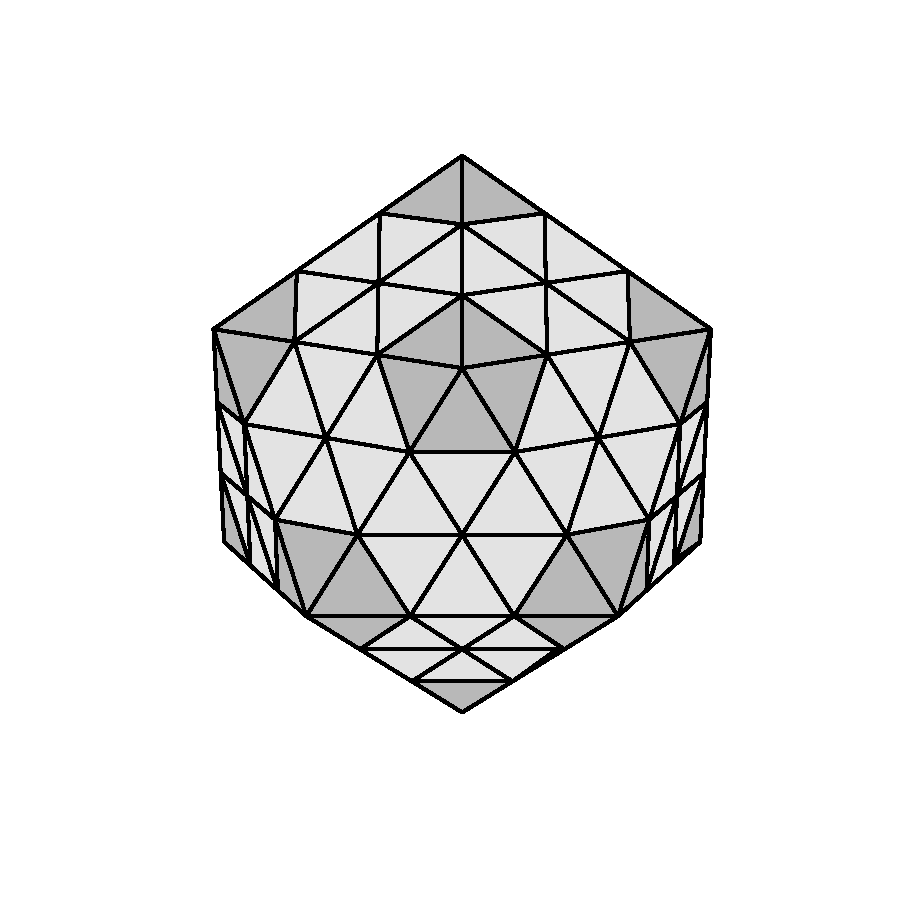
\includegraphics[height=3.5cm]{./figures/general_networks/full92_iso.pdf}
         \caption{Subdivided icosahedron.}
         \label{fig:topo1}
     \end{subfigure}
     \hfill
     \begin{subfigure}[b]{0.3\textwidth}
         \centering
         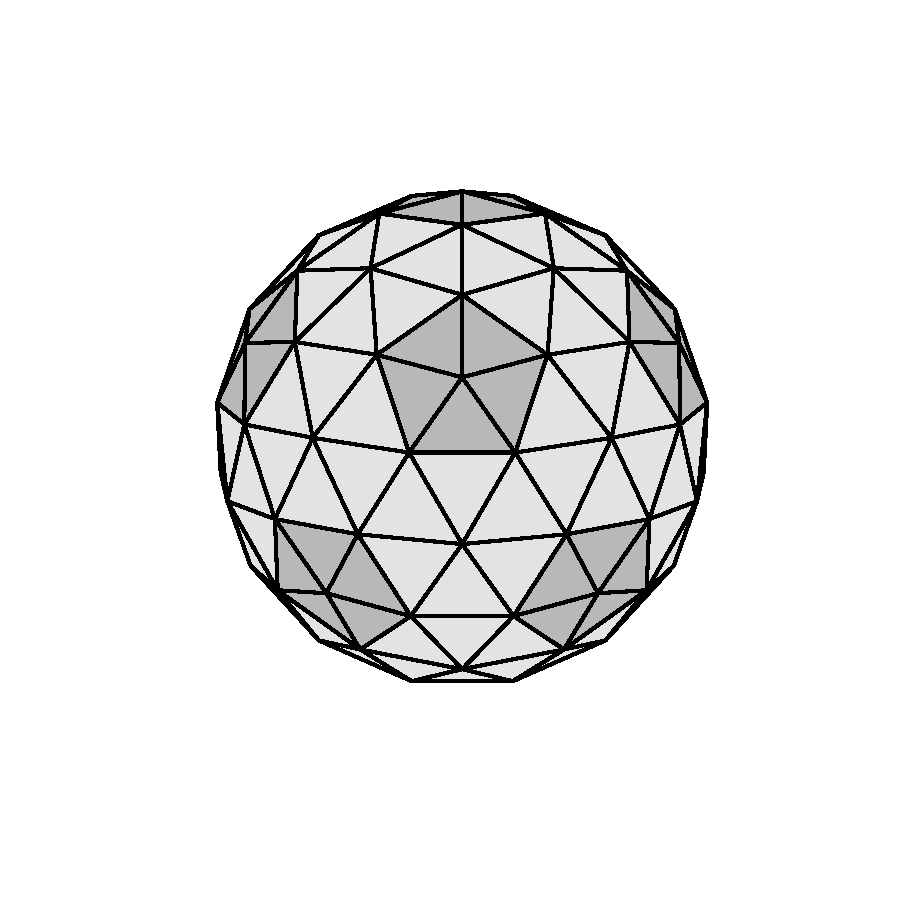
\includegraphics[height=3.5cm]{./figures/general_networks/full92_iso_min.pdf}
         \caption{Projected icosahedron.}
         \label{fig:topo2}
     \end{subfigure}
     \hfill
     \begin{subfigure}[b]{0.3\textwidth}
         \centering
         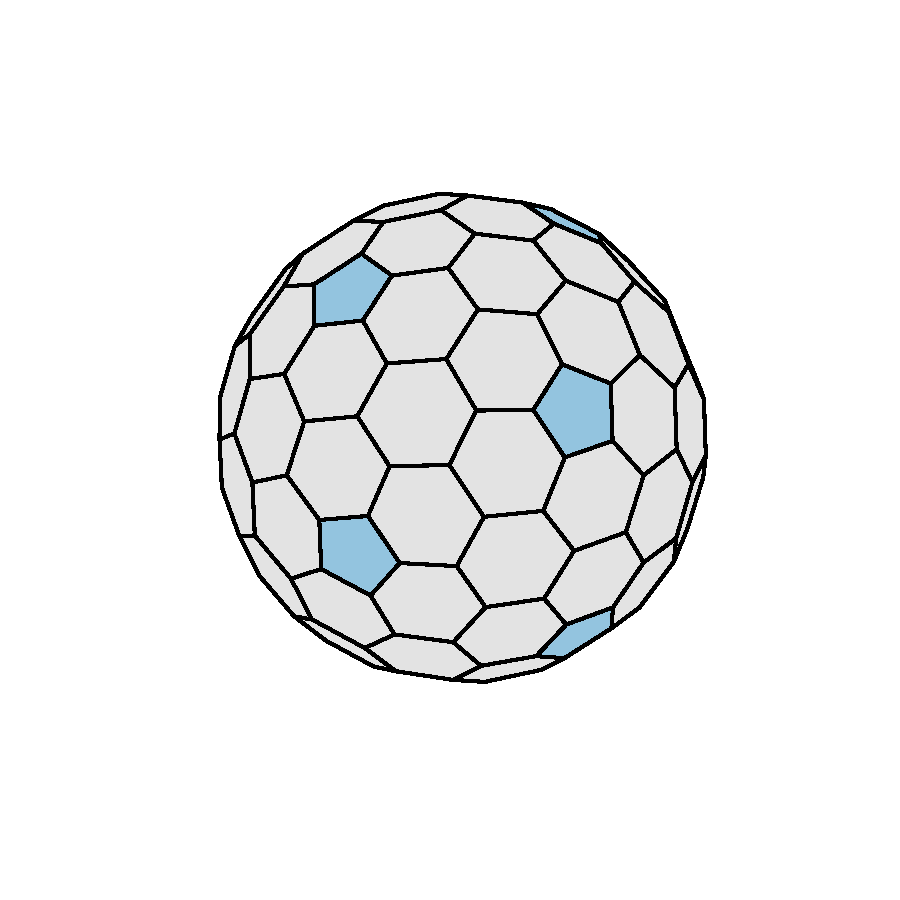
\includegraphics[height=3.5cm]{./figures/general_networks/full92.pdf}
         \caption{3\--coordinate fullerene}
         \label{fig:topo3}
     \end{subfigure}
     \hfill
     
     \vspace{0.2cm}
     \begin{subfigure}[b]{0.3\textwidth}
         \centering
         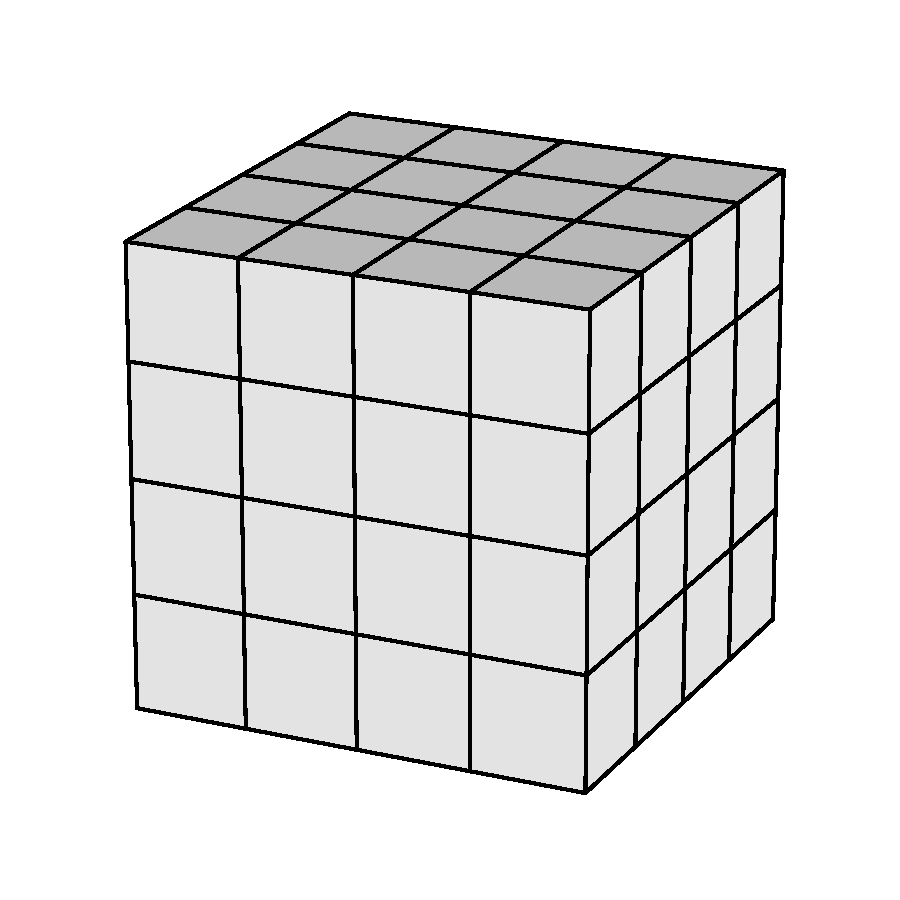
\includegraphics[height=3.5cm]{./figures/general_networks/full98_iso.pdf}
         \caption{Subdivided cube.}
         \label{fig:topo4}
     \end{subfigure}
     \hfill
     \begin{subfigure}[b]{0.3\textwidth}
         \centering
         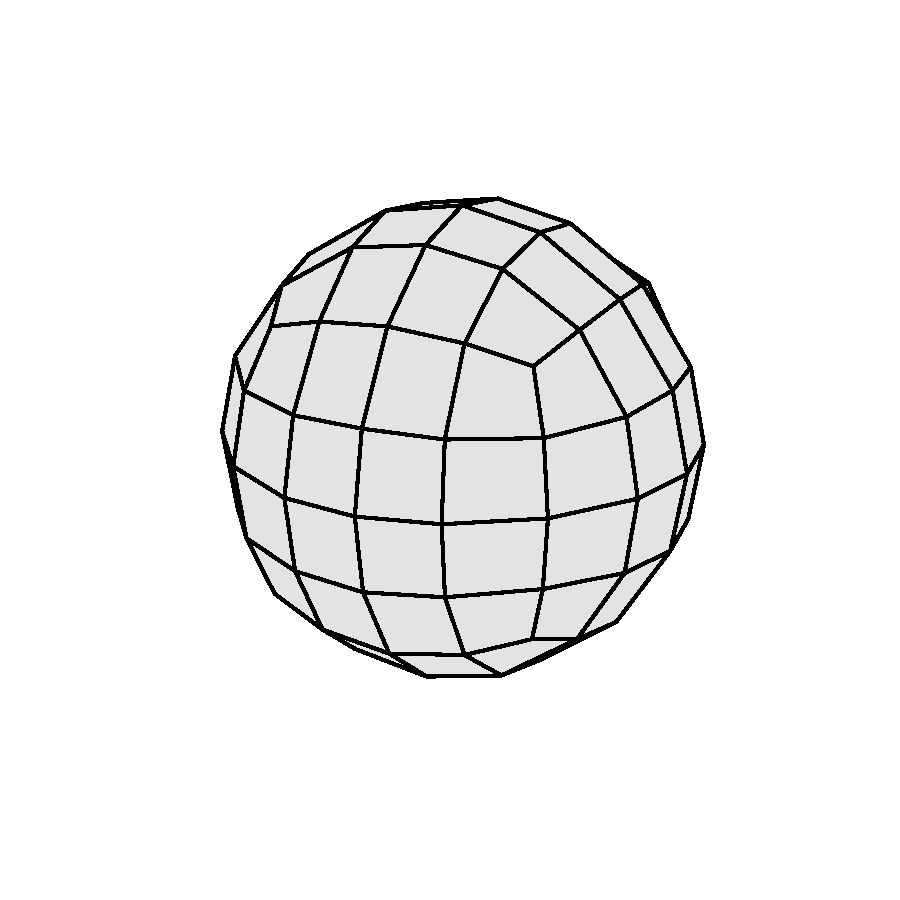
\includegraphics[height=3.5cm]{./figures/general_networks/full98_iso_min.pdf}
         \caption{Projected cube.}
         \label{fig:topo5}
     \end{subfigure}
     \hfill
     \begin{subfigure}[b]{0.3\textwidth}
         \centering
         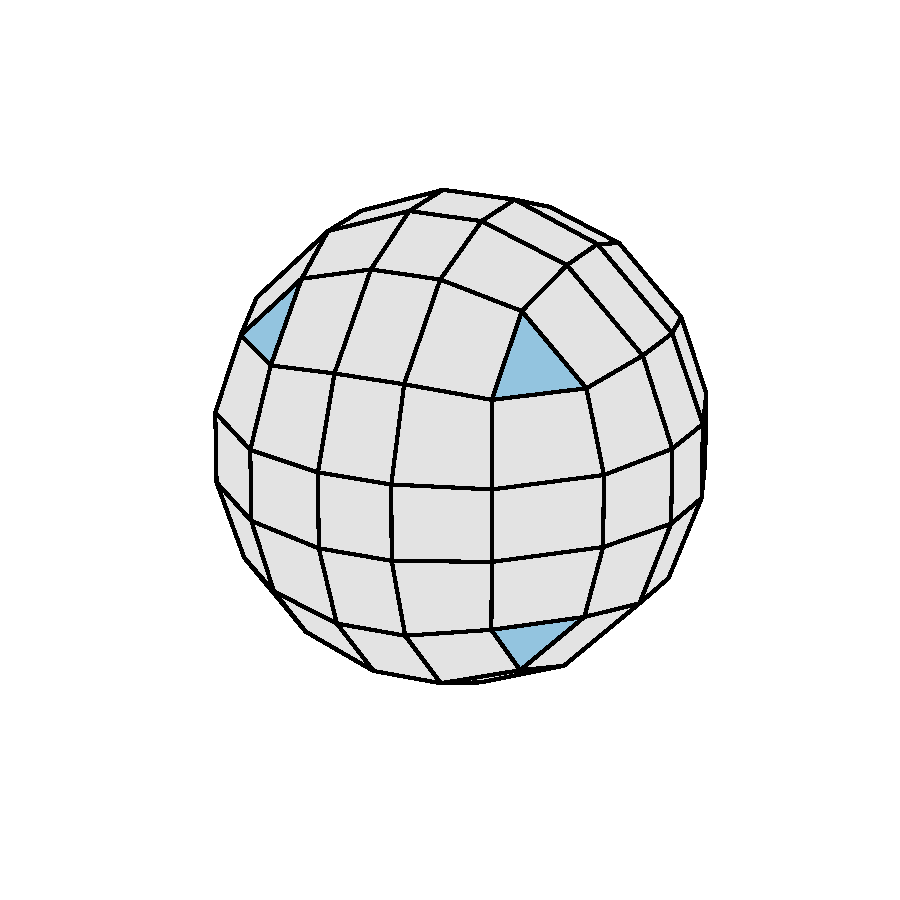
\includegraphics[height=3.5cm]{./figures/general_networks/full98.pdf}
         \caption{4\--coordinate fullerene.}
         \label{fig:topo6}
     \end{subfigure}
     \hfill
     
     \vspace{0.2cm}
     \begin{subfigure}[b]{0.3\textwidth}
         \centering
         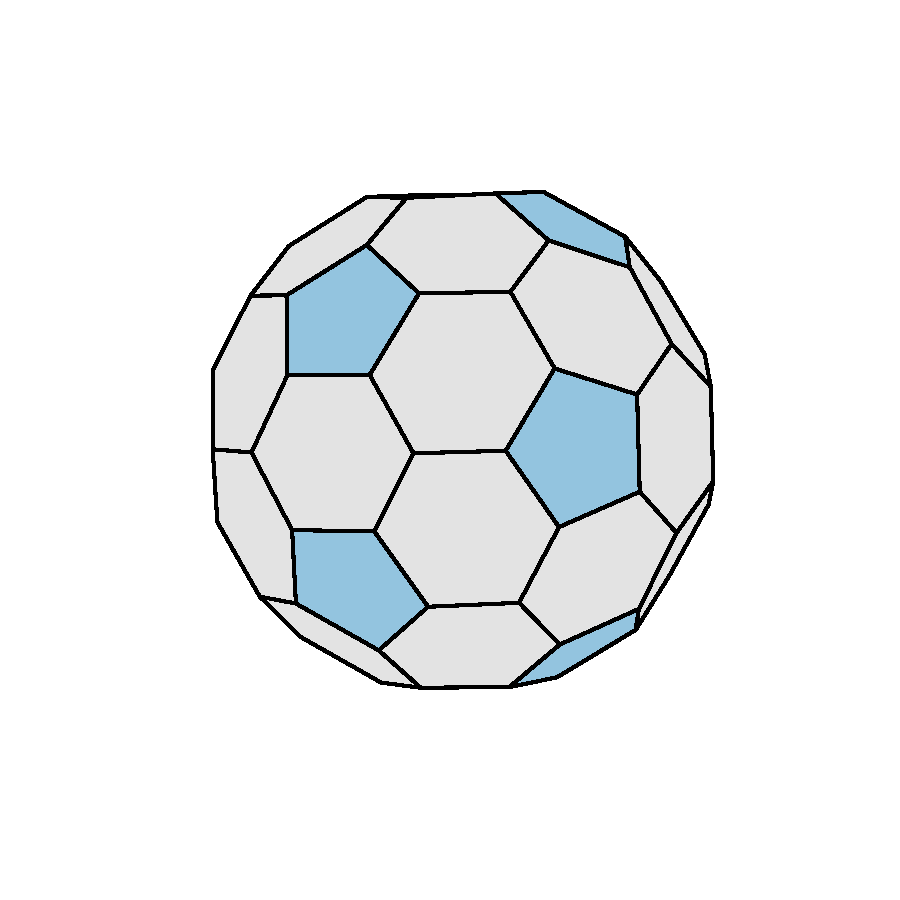
\includegraphics[height=3.5cm]{./figures/general_networks/full42.pdf}
         \caption{42\--ring fullerene.}
         \label{fig:topo7}
     \end{subfigure}
     \hfill
     \begin{subfigure}[b]{0.3\textwidth}
         \centering
         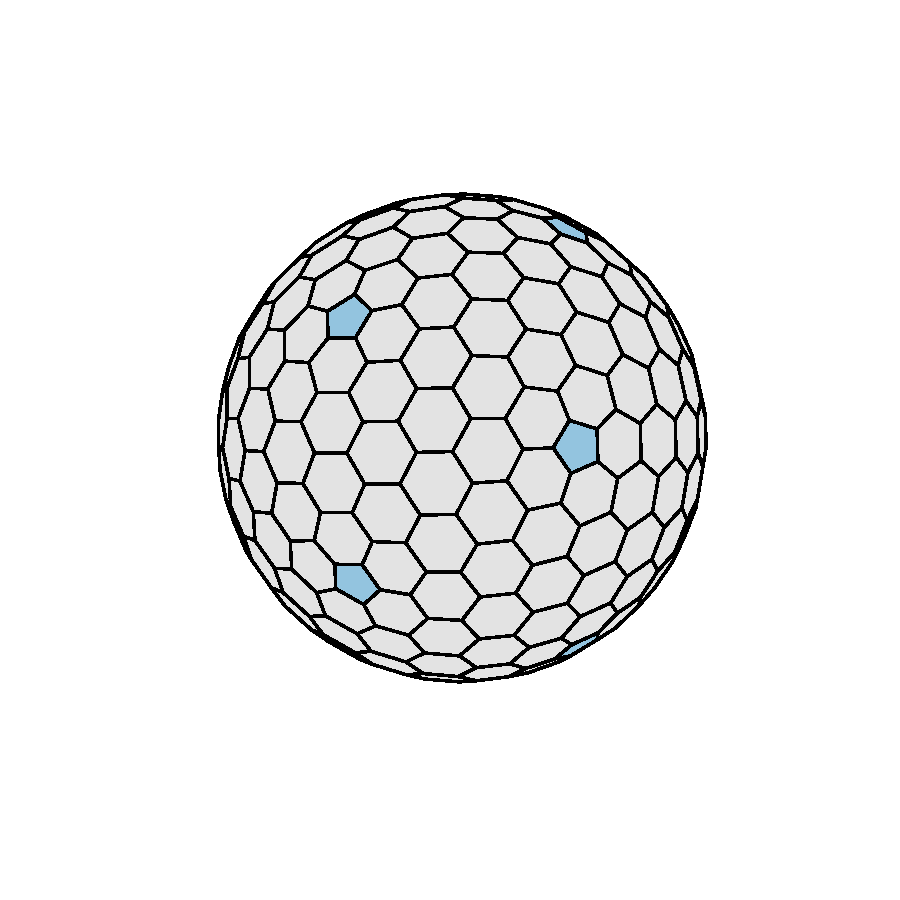
\includegraphics[height=3.5cm]{./figures/general_networks/full252.pdf}
         \caption{252\--ring fullerene.}
         \label{fig:topo8}
     \end{subfigure}
     \hfill
     \begin{subfigure}[b]{0.3\textwidth}
         \centering
         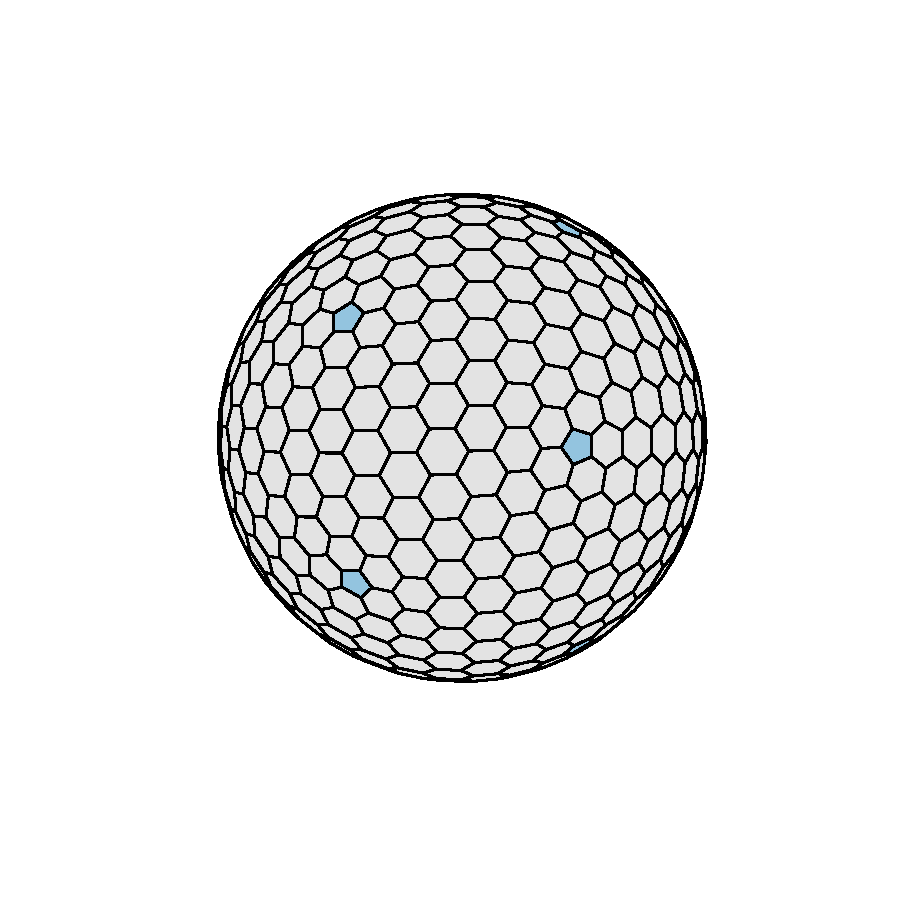
\includegraphics[height=3.5cm]{./figures/general_networks/full492.pdf}
         \caption{492\--ring fullerene.}
         \label{fig:topo9}
     \end{subfigure}
     \hfill
     
     \caption{Lattices of given coordination in spherical topology can be generated from the dual of a subdivided platonic solid, projected onto a sphere. Figures (a)\--(c) show this process for the icosahedron, giving a 3\--coordinate lattice and (d)\--(f) for the cube, giving a 4\--coordinate lattice. Altering the number of subdivisions allows the number of rings in the fullerene to be controlled.}
     \label{fig:topomethod}
\end{figure}

A further question that must be addressed is how to handle the potential model in spherical topology. 
One could implement all the potentials using spherical polar coordinates, which would strictly enforce the system topology.
However, here a simpler solution was used, whereby a simple harmonic restraining potential was between all atoms and the surface of the sphere, and the standard potential was used in three dimensional Euclidean space.
The atoms are therefore approximately maintained on a sphere of a fixed radius.
The radius is selected before the bond switching routine commences, corresponding to the minimum energy structure for the initial fullerene.

It is noted here that extensions to other topologies are certainly possible, albeit with varying degrees of difficulty.
All that is required is generation of a lattice which satisfies the underlying topological constraints, and an adequate potential model.
For example, a relatively easy extension would be to toroidal topology.
As previously mentioned, the periodic \td{} lattice has the same topology as the torus, and so there is a trivial mapping between the two (which is also the case for a M\"obius strip and Klein bottle, although these currently seem less chemically relevant).
Application to systems with a larger number of topological holes would however require a different method to generate the initial lattice. 

\section{List of Studied Networks}

In this chapter data on networks will be presented from a range of different sources, covering both computation and experiment.
These are detailed here as a reference for the remainder of the chapter.

\subsection{Computational Networks}
\label{s:gennetcompsamples}

All networks derived from computation were calculated using methods described in this thesis.
They are as follows:
\begin{enumerate}
	\item \textbf{Bond switching}: networks of $1024$ rings for $\ki=4,6$ and $1152$ rings for $\ki=5$. 
	In a simulation, the system was thermalised with $2\times 10^5$ random moves, and annealed over a further $4\times 10^6$ moves. 
	A series of different potential models were also used with bond length/angle force constant ratios of $k_r/k_\theta=16,4,1,1/4$. 
	For each parameter set, 100 simulations were run starting from different random seeds.
	\item \textbf{Triangle rafts}: networks of $1000$ rings across a temperature range of $T=10^{-4.5}\rightarrow10^{-1.5}$, as outlined in section \ref{s:triangleraft}, totalling some $27,500$ configurations.  
	\item \textbf{Hard disk \mc}: systems of $1000$ disks at packing fractions in the range $\phi=0.0\rightarrow0.77$.
	Each simulation comprised cycles of $1000$ random displacement moves, with $10^5$ equilibration cycles, $10^5$ production cycles and with sampling every 10 production cycles. 
	For each packing fraction 10 simulations were run using a different random seed.
	 A Voronoi analysis was performed for each configuration to generate a system of tessellating rings, as discussed in section \ref{s:hardparticlemc}.
\end{enumerate} 

\subsection{Experimental Networks}
\label{s:genexpnetworks}

Comparison is also made to a variety of experimental networks obtained from a variety of publications.
They are as follows:
\begin{enumerate}
	\item \textbf{Colloidal monolayers}: particles with a diameter of $\sim 2.79~\mu$m dispersed in a water\--ethanol mixture and confined by gravity to form a monolayer on the base of a glass sample cell, with packing fractions in the range $\phi=0.29\rightarrow 0.66$ \cite{Thorneywork2017}.
Out\--of\--plane fluctuations are quantified by the gravitational height of the particles, which is a very small percentage of their diameter, and as such the system is structurally two-dimensional.
Each packing fraction has 100 associated frames, with the time between frames around 10s.
At the highest packing fractions considered, the area of the system imaged contains around 3000 particles.
As the system is aperiodic, after Voronoi analysis the cells on the image boundary are neglected.
\item \textbf{Silica bilayers}: configurations of thin films of silica glass grown on graphene \cite{Huang2012} and Ru(001) \cite{Buchner2017}.
Three samples were obtained consisting of 291, 444 and 446 rings.
\item \textbf{Amorphous graphene}: configurations of graphene amorphised by irradiation with an electron beam \cite{Eder2014}.
Exposure to increasing doses created 14 samples with varying levels of disorder.
For each sample, defects were identified from the presence of under\--coordinated atoms, arising largely from the sample perimeter or from holes in the centre, which were removed.
After processing, configurations comprised $\sim3000\rightarrow5000$ rings.
\item \textbf{Geopolitical regions}: physicists have previously studied the regions of France and Ireland, and noted the similarity in their properties to materials \cite{LeCaer1993,Okabe1992}.
This tradition has been continued by analysing five further maps: the communes of Switzerland, the parishes and Westminster constituencies of Great Britain and the socio\--economic regions of the European Union (EU) and the European Free Trade Association (EFTA) (including both current and candidate countries at the time of writing) \cite{osmap,chmap,eumap}. Details of the analysis can be found in appendix \ref{app:maps}.
\end{enumerate}

\section{Investigations into Generic Physical Networks}

The properties \td{} atomic networks are now discussed alongside generic physical systems introduced in this chapter.
This primarily focusses on the network properties introduced in chapter \ref{ch:networktheory}, but also covers a case study on the energetics of a 92\--ring fullerene.

\subsection{Degree Distributions}
\label{s:gendegreedist}

The degree distributions of physical networks are discussed in terms of Lemaitre's law; with the distribution variance, $\mu_2$, plotted against the proportion of rings of mean size.
Figure \ref{fig:lmgena} presents these data for a range of 3\--coordinate systems comprising experimental, computational and theoretical.
There are many things to note, but primarily it can be seen that regardless of the nature of the underlying system, all data fit very well with the maximum entropy solution provided by \lm{}'s law.
Whilst \lm's law highlights the similarities between these systems, it is also important to examine some of their differences. For example, what determines where a system sits on the \lm{} curve \ie{} what controls the number of hexagons?
For materials this is based on energetics \-- the strain associated with bond and angle distortions. For instance, experimentally silica bilayers have more diverse ring statistics than graphene owing to the reduction in ring strain due to the presence of oxygen linkages\cite{Buchner2017}.
Even for the graphene samples which have been modified by an electron beam (pink diamonds), the disorder does not approach that of the silica glasses (orange hexagons).
For the colloid systems (blue circles) however, the rings are formed from the Voronoi tessellation, with no intrinsic cost to distortions and instead it is the packing fraction, $\phi$, which determines $p_6$.
The limit $\phi\rightarrow 0$ achieves the Poisson Voronoi ring distribution (yellow star) \cite{Tanemura2003}, with a lower bound of $p_6 \approx 0.295$.
For for the administrative geopolitical regions, there is no energy cost for rings, regardless of shape, convexity or separation, and so we find these points (red triangles) in the low $p_6$, high entropy portion of \lm's{} curve.

On the other hand, using a flexible computational method allows access to the entire range of $\mu_2$ values, where the level of disorder is controlled by the Monte Carlo ``temperature'' parameter.
The results from bond switching highlight the typical dispersion that can be expected within \lm's{} law, with the grey shaded region indicating the bounds of $\mu_2$ within two standard deviations of the mean.
Finally it can be seen that using equation \eqref{eq:mer} with the $p_6$ and $r$ values from hard disk Monte Carlo (blue dashed line) reproduces the results from \lm's{} law without the need for the empirical constraint.
The calculation of this line is explained at the end of section \ref{s:genassortativity}.

\begin{figure}[bt]
     \centering
     
      \begin{subfigure}[b]{0.45\textwidth}
         \centering
         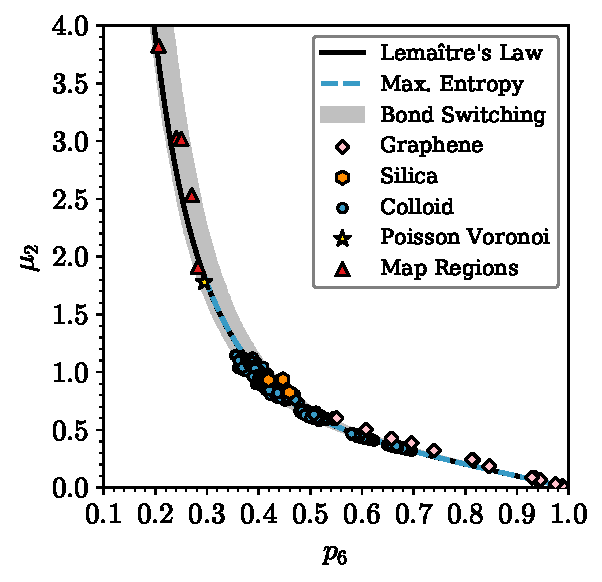
\includegraphics[width=\textwidth]{./figures/general_networks/gen_lm.pdf}
         \caption{SK potential, $c=3$}
         \label{fig:lmgena}
     \end{subfigure}
     \hfill
     
     \begin{subfigure}[b]{0.45\textwidth}
         \centering
         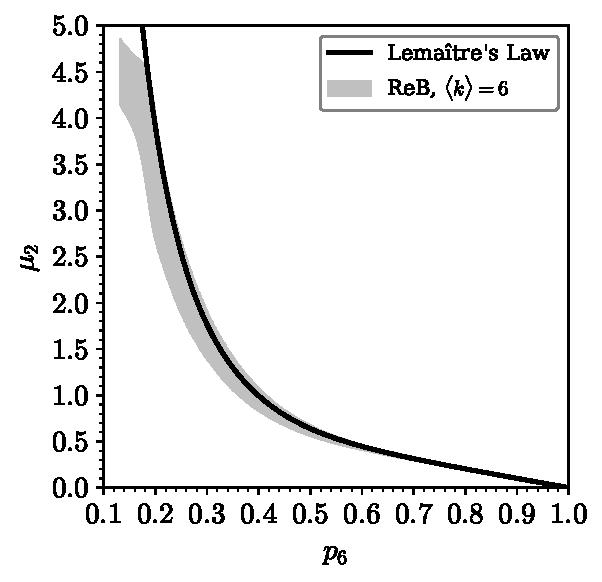
\includegraphics[width=\textwidth]{./figures/general_networks/lemaitre_6.pdf}
         \caption{ReB potential, $c=3$}
         \label{fig:lmgenb}
     \end{subfigure}
     \hfill
     \begin{subfigure}[b]{0.45\textwidth}
         \centering
         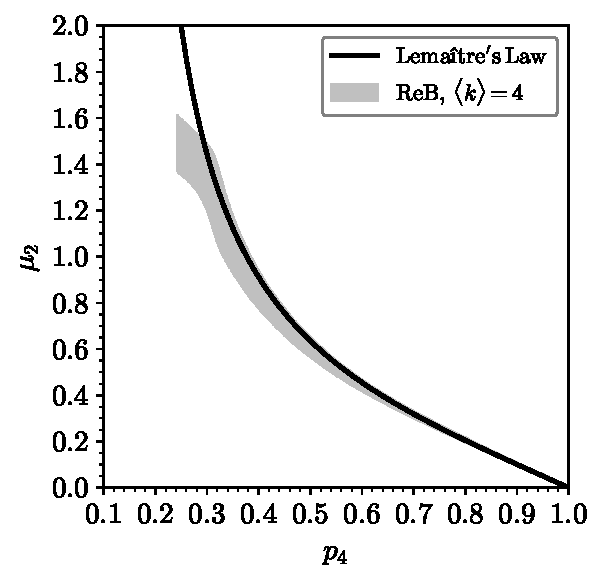
\includegraphics[width=\textwidth]{./figures/general_networks/lemaitre_4.pdf}
         \caption{ReB potential, $c=4$}
         \label{fig:lmgenc}
     \end{subfigure}
     \hfill
 
     \caption{Physical networks are shown to agree well with \lm's law. Panel (a): \lm's law (black line) is compared to to bond switching simulations of 3\--coordinate \td{} materials (grey area representing two standard deviations from the mean), amorphous graphene (pink diamonds), silica bilayers (orange hexagons), colloidal monolayers (blue circles), the Poisson Voronoi diagram (yellow star) and maps of geopolitical regions (red triangles). Panels (b) and (c): comparison to bond switching with ring convexity maintained using the ReB potential for 3\-- and 4\--coordinate systems respectively.}
     \label{fig:lmgen}
\end{figure}

The effect on the maximum entropy solutions can also be explored for different atomic coordination environments and constraints.
Figures \ref{fig:lmgenb} and \ref{fig:lmgenc} gives two such examples where ring convexity is enforced by using the ReB potential.
Figure \ref{fig:lmgenb} gives results for a purely 3\-- coordinate system, $x_3=1$, whilst figure \ref{fig:lmgenc} gives results for a purely 4\-- coordinate system, $x_4=1$.
The maximum entropy solution each case is again given by equation \eqref{eq:mepk}, with $\ki=6,4$ respectively.
The value of $\mu_2$ is very similar for $\ki=4$ and $\ki=6$ above $p_{\ki}\approx 0.5$.
This is because in this region rings of sizes $k=\ki$ and $k=\ki\pm1$ dominate the distribution and so $\mu_2\approx 1-p_{\ki}$.
However, as the value of $p_{\ki}$ is reduced further, the two maximum entropy curves begin to diverge as the $k=\ki-2$ ring becomes accessible only to the 3- coordinate system, which in turn facilitates the presence of higher order rings.
In both cases, the results from bond switching both begin to deviate from the analytical results of \lm's{} law at low $p_{\ki}$.
The origins of this deviation can be traced back to the fact that if ring convexity is strictly maintained, it becomes increasingly difficult to accommodate the very large rings required to achieve large $\mu_2$ values.


\subsection{Assortativity}
\label{s:genassortativity}

The ring correlations as measured by the assortativity are given for all 3\-- coordinate systems in figure \ref{fig:assortgena}.
It is found that all these 3\-- coordinate networks are disassortative and lie in the region $-0.35<r<-0.10$ and that curves display a similar characteristic shape.
The experimental colloid samples are well described by the hard disk model (blue points and line), with $p_6\approx0.84$ corresponding to packing fractions above the freezing transition limit ($\phi\approx 0.70$) \cite{Bernard2011}.
The curves generated from bond switching and triangle rafts display different assortativities which depend on the balance of the length\-- and angle\--drive forces.
The driving force for the hard disk model is purely entropic, whereas for the other methods there is also a complex energy landscape, which may favour specific assortativities and which can be ``tuned'' by altering the balance of the interactions. 
For example the bond switching results show the effect of varying this balance with $k_r/k_\theta=16,4,1,1/4$ (black to light grey lines), leading to a shifting in the assortativity curves.
This is supported by the experimental results from amorphous graphene (pink diamonds), which lie in the between the two curves with the largest bond length to angle force constant ratio, as would be intuitively expected for atomic systems and from empirical potential models \cite{Kumar2012}.

\begin{figure}[bt]
     \centering
     
      \begin{subfigure}[b]{0.45\textwidth}
         \centering
         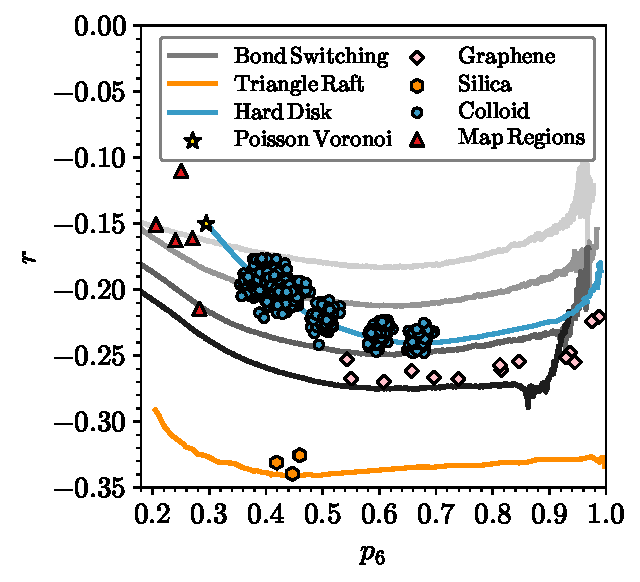
\includegraphics[width=\textwidth]{./figures/general_networks/gen_assort.pdf}
         \caption{Assortativity.}
         \label{fig:assortgena}
     \end{subfigure}
     \hfill
     
	\vspace{0.5cm}     
     \begin{subfigure}[b]{0.2\textwidth}
         \centering
         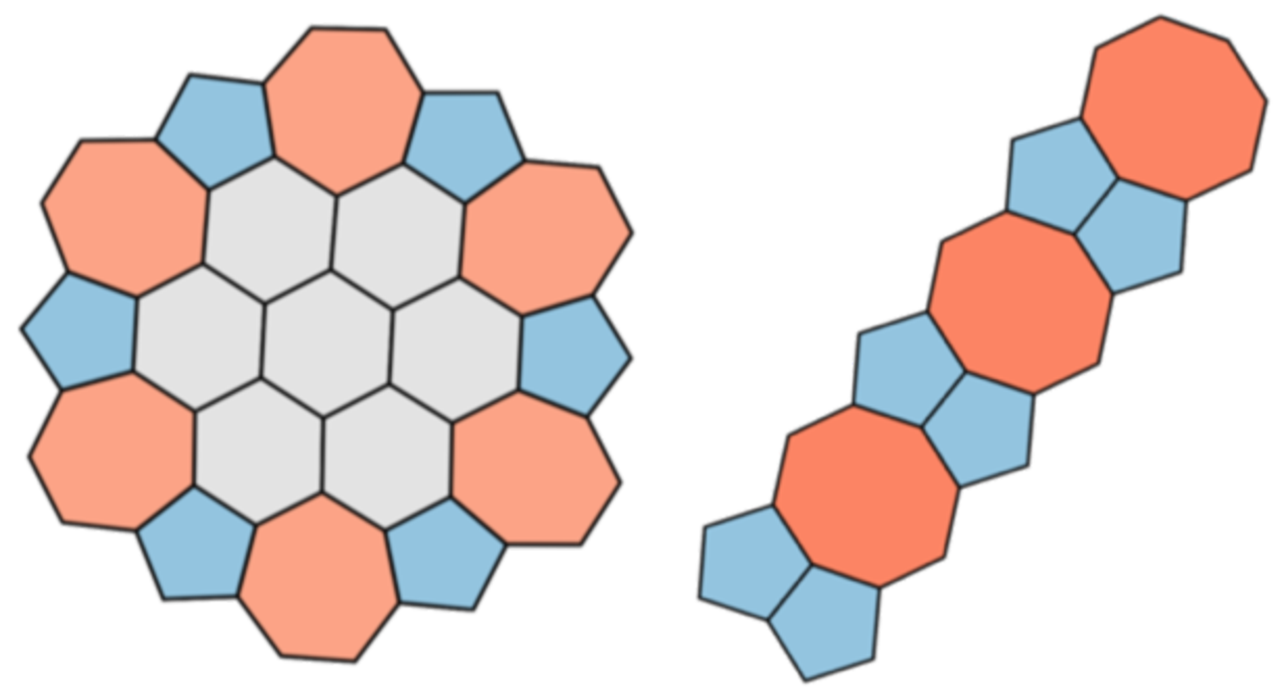
\includegraphics[height=2cm]{./figures/general_networks/defect_-33.pdf}
         \caption{$r=-0.\dot{3}$}
         \label{fig:defect33}
     \end{subfigure}
     \hfill
   \begin{subfigure}[b]{0.2\textwidth}
         \centering
         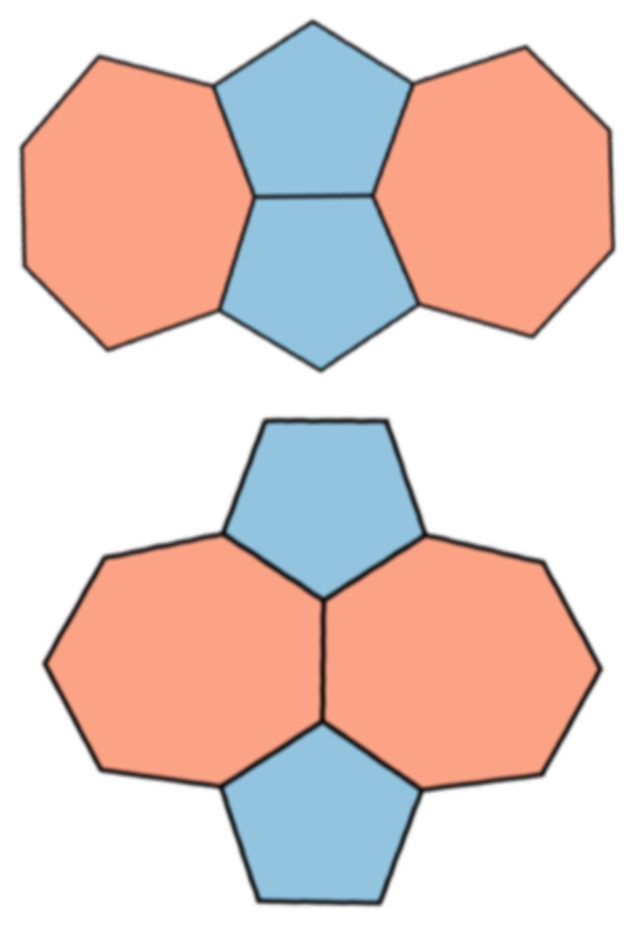
\includegraphics[height=2cm]{./figures/general_networks/defect_-25.pdf}
         \caption{$r=-0.25$}
         \label{fig:defect25}
     \end{subfigure}
     \hfill
     \begin{subfigure}[b]{0.2\textwidth}
      \centering
     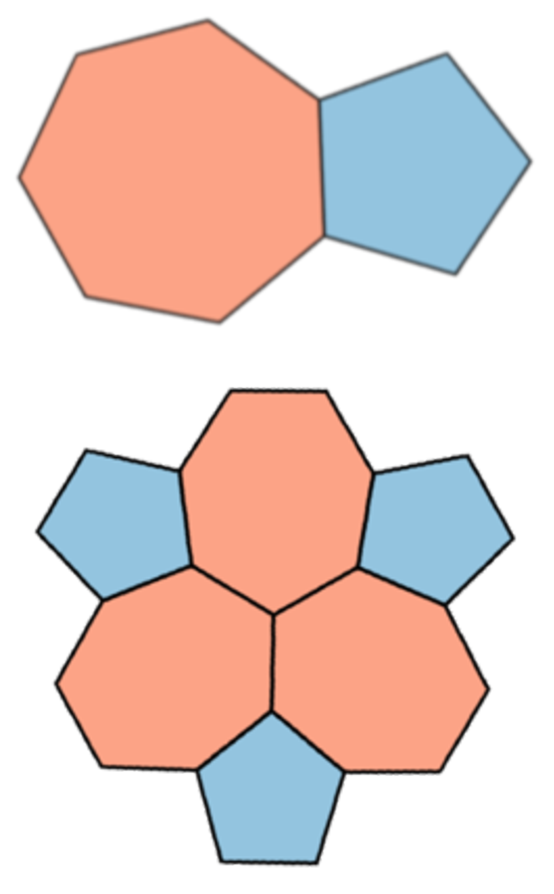
\includegraphics[height=2cm]{./figures/general_networks/defect_-17.pdf}
         \caption{$r=-0.1\dot{6}$}
         \label{fig:defect17}
     \end{subfigure}
     \hfill
     \begin{subfigure}[b]{0.2\textwidth}
      \centering
     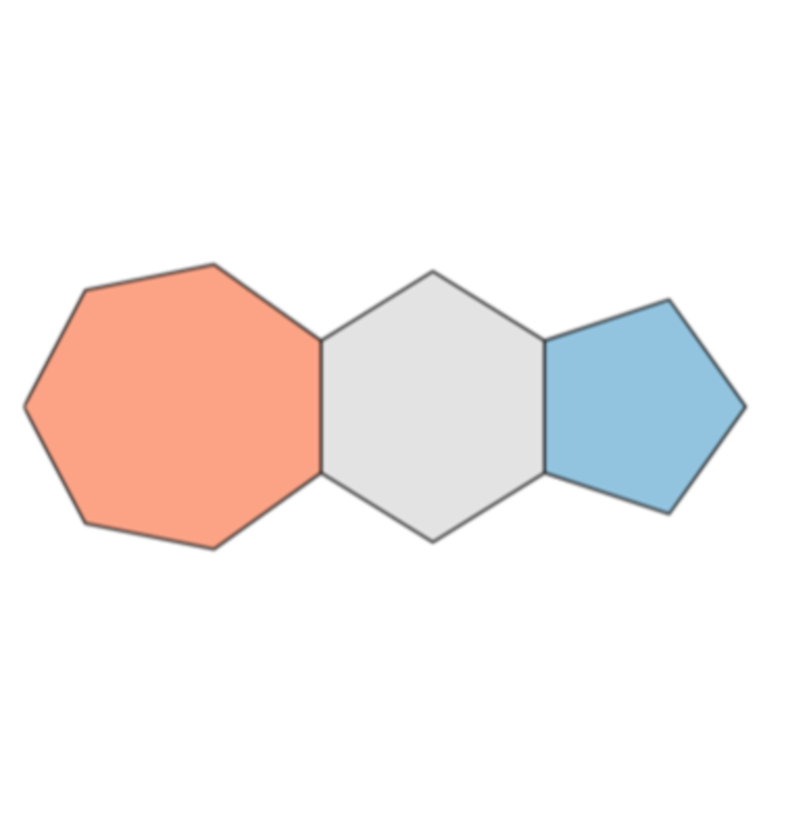
\includegraphics[height=2cm]{./figures/general_networks/defect_0.pdf}
         \caption{$r=0.0$}
         \label{fig:defect0}
     \end{subfigure}
     \hfill
   
     \caption{Panel (a): variation in assortativity, $r$, against $p_6$ for a range of 3\--coordinate systems comprising experimental and simulation data. For bond switching data, darker grey colouring indicates a greater $k_r/k_\theta$.
Panels (b)\--(e) show common defects found in crystalline systems, with their limiting assortativity value (b) isolated pair, $r=0.0$; (c) adjacent pair, cluster, $r=-0.1\dot{6}$;  (d) Stone\--Wales, mitosis, $r=-0.25$;  (e) 5\--7 chain (flower defect), 5\--8 chain, $r=-0.\dot{3}$.}
     \label{fig:assortgen}
\end{figure}

For all the systems we note that there are different regimes, with the high $p_6$ limit corresponding to configurations best described as crystalline with defects rather than truly amorphous as in the low $p_6$ limit \-- with the two often being linked by a phase transition.
The high $p_6$ limit can be rationalised by considering the frequency of common defect types at infinite dilution in a hexagonal lattice \cite{Marcus1997,Bjorkman2013} (figure \ref{fig:defect33}\--\ref{fig:defect0}).
These can be calculated by considering the explicit edge joint probability distribution for a specific defect.
For example, for the Stone\--Wales defect \ref{fig:defect25}, each 5\--ring has two 7\--ring neighbours, and each 7\--ring two 5\--ring and one 7\--ring neighbours such that:
\begin{equation}
        \mathbf{e} = \begin{blockarray}{*{3}{c} l}
        \begin{block}{*{3}{>{$\footnotesize}c<{$}} l}
        5 & 6 & 7 \vspace{-1mm}\\
        \end{block}
        \begin{block}{[*{3}{c}]>{$\footnotesize}l<{$}}
        \:0 & 3\delta & 2\delta \: \bigstrut[t]& \:5\\
        3\delta & 1-19\delta & 4\delta & \:6 \\
        2\delta & 4\delta & \delta & \:7\\
        \end{block}
        \end{blockarray}
\end{equation}
where $\delta=\left(1-p_6\right)/12$.
From here it is straightforward to evaluate the dilute $p_6$ limit as $\lim\limits_{\delta\rightarrow 0} r = \frac{1}{4}$.

This helps to rationalise the high $p_6$ disassortative behaviour for these 3\--coordinate systems.
For hard disks as $p_6\rightarrow 1$ the adjacent pair appears to be dominant, whereas for bond switching and triangle rafts the potential model determines the balance of defect types.
For bond switching the standard deviation is large as each sample contains a single defect corresponding to one of the low energy forms.
By visual inspection, increasing the length relative to the angle driving force preferences chain\--like structures over isolated defects.
Similarly the rigidity of the triangle units in the triangle raft method leads to a very tight length distribution which encourages the formation of defects such as \ref{fig:defect0}.
As $p_6$ decreases more defects are introduced and the system becomes truly amorphous.
Again one can posit that as the hard disk model has no energetic term, it is able to incorporate less correlated defects, and in the low packing fraction the hard disk model provides an estimate for the Poisson Voronoi limit of $r\approx-0.15$.

Again the effects of coordination environment and potential model on assortativity in complex networks can be demonstrated using bond switching.
Figure \ref{fig:assortmixa} shows such a comparison, where the assortativity is plotted against the primary ring size for different coordination environments, averaged by Monte Carlo temperature.
The effect of imposing a hard constraint on ring convexity can be seen through the two curves corresponding to $\ki=6$.
These curves show very similar behaviour for $p_6\gtrsim0.3$, below which there is increasing deviation.
This is as expected given the violation of ring convexity will only occur for very large rings at high temperatures, which can undergo deformation to reduce bond angle strain.
This allows larger rings to pack next to each other, reducing the disassortativity.
The behaviour of the pure 4\--coordinate system, $\ki=4$, is qualitatively the same as for the 3\--coordinate network, and indeed all the defects in figure \ref{fig:assortgen} have analogues in 4\--coordinate networks.
The network of greater interest is that with mixed 3\-- and 4\--coordinate vertices, corresponding to $\ki=5$.
In this case one can see fundamentally different properties as these networks are assortative at high $p_5$, in contrast to limiting pure coordination cases.
This assortative mixing is readily explainable through energetic considerations.
The hexagonal and square tilings are strainless and so the disruptive effects of any defect rings is minimised when such rings are adjacent.
Unlike the hexagonal and square lattices, the Cairo lattice is not strainless, due to a distortion in one of the edge lengths in the pentagonal tiles.
Therefore, any 4- or 6-ring defects experience a driving force to cluster into the low energy regular tilings.
In effect the lattice de\--mixes into Cairo, square and hexagonal regions (as in figure \ref{fig:assortmixb}), which can be identified as inherently assortative behaviour.
It is for this same reason that the limit of $p_5\rightarrow 1$ cannot be reached, as the minimum energy lattice will be a mixture of the square, hexagonal and Cairo lattices, the exact proportion of which will depend on the potential model.

\begin{figure}[bt]
     \centering
     
      \begin{subfigure}[b]{0.45\textwidth}
         \centering
         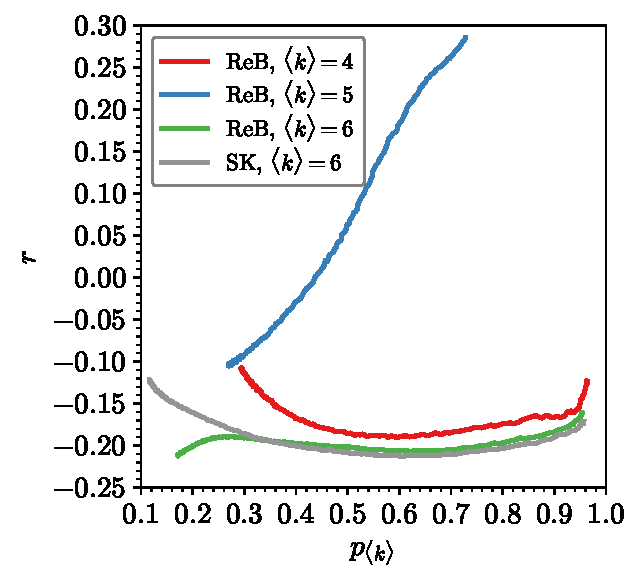
\includegraphics[width=\textwidth]{./figures/general_networks/mix_assort.pdf}
         \caption{}
         \label{fig:assortmixa}
     \end{subfigure}
     \hfill
     \begin{subfigure}[b]{0.45\textwidth}
         \centering
         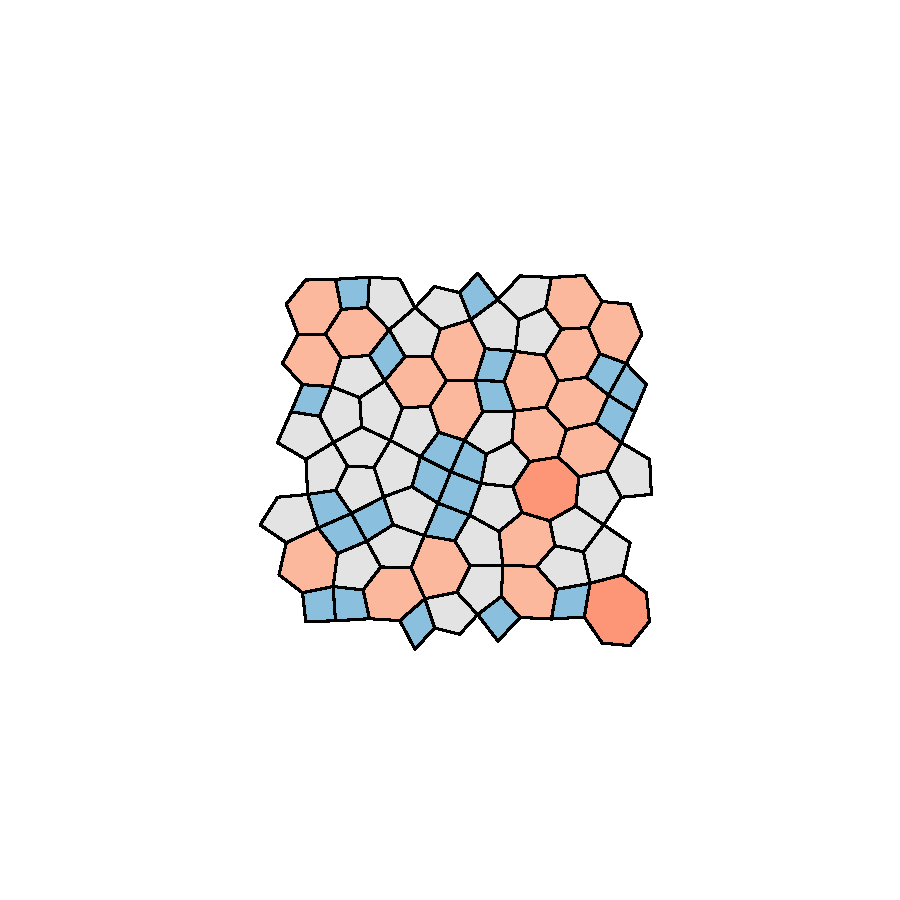
\includegraphics[height=5cm]{./figures/general_networks/cairo.pdf}
         \caption{}
         \label{fig:assortmixb}
     \end{subfigure}
     \hfill
     
     \caption{Panel (a) shows the variation in assortativity, with ring statistics for 3\--coordinate (green, grey lines), 4\--coordinate (red line) and mixed 3/4\--coordination systems (blue line) using the simplified Keating (SK) and restricted bending (ReB) potentials as indicated. Panel (b) gives a small configuration of a mixed coordination lattice displaying clustering of rings of similar size.}
     \label{fig:assortmix}
\end{figure}

Finally the accuracy of the extension to \lm's maximum entropy method in equation \eqref{eq:mer} is assessed.
Calculation of the maximum entropy joint degree distribution requires two parameters, $p_6$ and $r$, but the resulting distribution contains all the information required to calculate ring statistics, $p_k$, and the mean ring size about each ring, $m_k$.
This has been performed using the parameters of $p_6$ and $r$ from hard disk simulations.
As demonstrated in figure \ref{fig:lmgena}, the ring statistics calculated in this way regenerate those from \lm's law.
In addition, plots of the mean ring sizes for selected packing fractions are given in figure \ref{fig:hdme}. Whilst the fit is not perfect, this method does provide a close approximation to the hard disk results, particularly in the vicinity of $k=\ki$. The results are especially good in the context that only two variables are required in $p_6$ and $r$ to generate the distributions.

\begin{figure}
\centering
        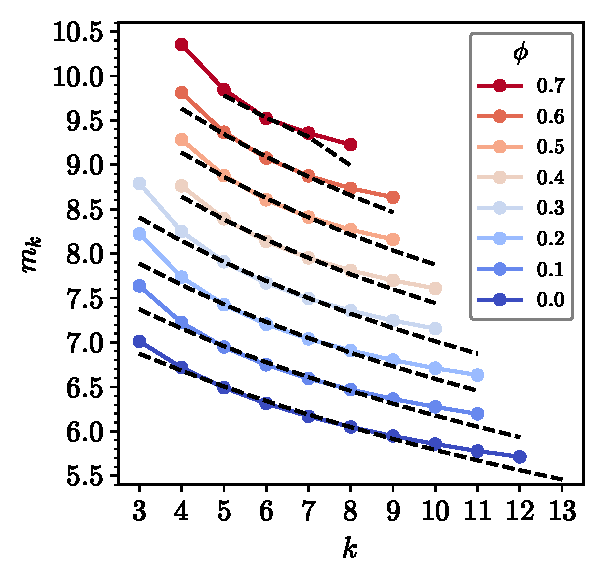
\includegraphics[width=7cm]{./figures/general_networks/hdme.pdf}
        \caption{Mean ring size of hard disk simulations at different packing fractions (full lines) compared to results from maximum entropy (dashed lines). In both cases only ring sizes with $p_k>10^{-4}$ are displayed and results are offset by $0.5$ along the abscissa for clarity.}
        \label{fig:hdme}
\end{figure}

\subsection{Energetics of Fullerenes}

As an illustration of the generalisability of the methods described in this work, results are presented for two\--dimensional networks in spherical topology.
Such systems are also of experimental interest, as experimentalists now have access to ``non-classical'' fullerenes\cite{Tian2019,Guan2019,Brotsman2017,Kemnitz2018}, metal-organic nano-cages\cite{Fujita2016,Wang2017} as well as curved froths \cite{Roth2012}.
One such fullerene was investigated here: a 92\--ring 3\--coordinate fullerene consisting of 5,6 and 7\-- rings.
Possible configurations were again generated via bond switching, starting from the lattice depicted in figure \ref{fig:topo3}.
Here $10^6$ total configurations were sampled from 100 different simulations, with $k_r/k_\theta=4$.

Results of the network properties averaged across configurations are given in figure \ref{fig:fullerene92u}, coloured by potential energy.
In this plot the value of $p_6$ is discretised, owing to the the small and well\--defined number of rings, and cannot exceed the upper limit imposed by the 12\--pentagon rule, whereas the assortativity is averaged.
As expected, the energy of the fullerenes increases with the increasing diversity in the ring statistics, as more pentagons and heptagons are accommodated.
However, it is also the case that the arrangement of the rings, as measured by the assortativity, is also very important in determining the stability of the networks.
To emphasise this, three example configurations are provided in figure \ref{fig:fullerene92a}\--\ref{fig:fullerene92c}.
These amorphous fullerenes have the same $p_6$ value (and therefore $p_5$, $p_7$), but very different strain energies.
In \ref{fig:fullerene92c} defects appear which are similar to the common motifs as in figure \ref{fig:assortgen} \ie{} those associated with being low energy.
The increased clustering of similar sized rings in \ref{fig:fullerene92a},\ref{fig:fullerene92b} leads to increasingly irregular ring geometries that generate high levels of strain.
As previously noted with planar networks, systems which are disassortative are energetically favoured.
Although this is a simple consequence of the mechanical properties of the system, neglecting any electronic contributions, such is the difference in stability that we would expect disassortative fullerenes of this type to be more prevalent in nature.

\begin{figure}[bt]
     \centering
      \begin{subfigure}[b]{0.45\textwidth}
         \centering
         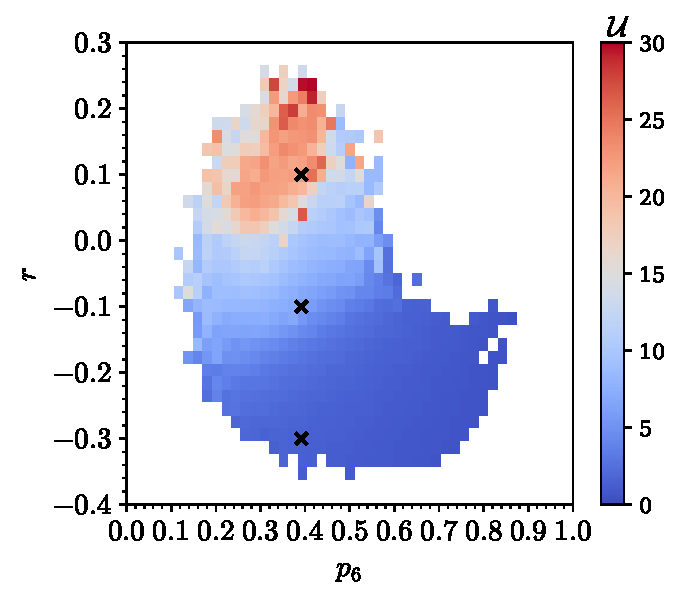
\includegraphics[width=\textwidth]{./figures/general_networks/energy_full92.pdf}
         \caption{}
         \label{fig:fullerene92u}
     \end{subfigure}
     \hfill
     
	\vspace{0.5cm}     
     
     \begin{subfigure}[b]{0.22\textwidth}
         \centering
         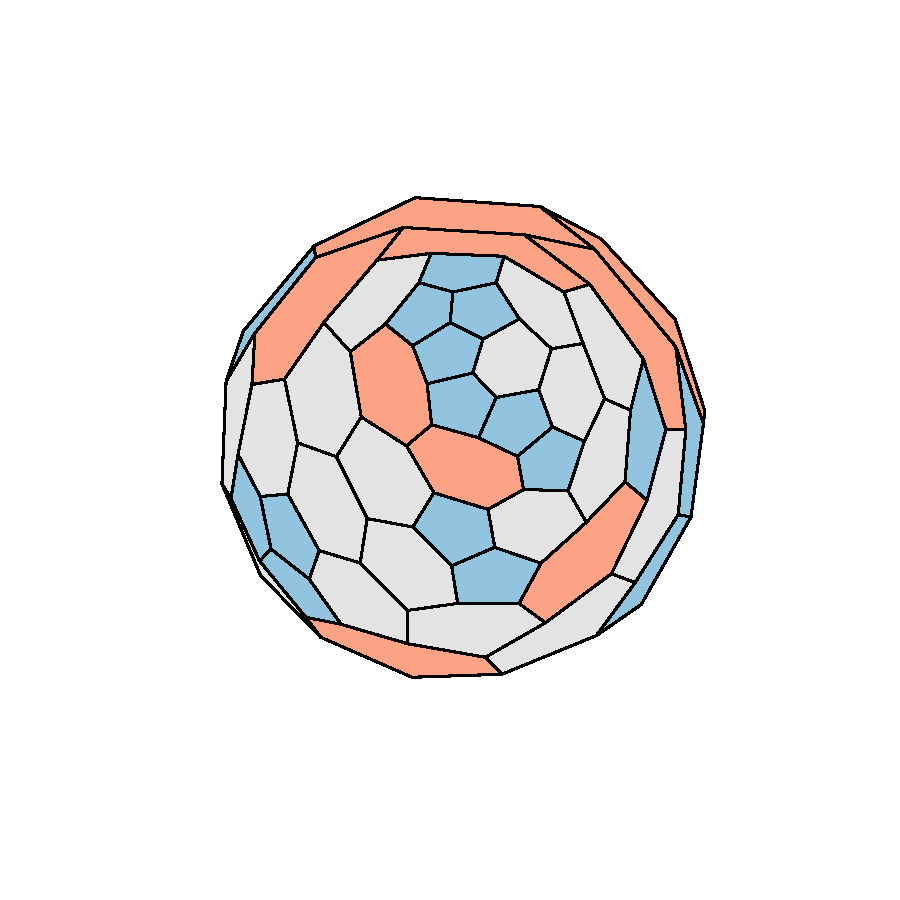
\includegraphics[width=\textwidth]{./figures/general_networks/full92_r10.pdf}
         \caption{$p_6=36/92$,\\ $r=0.1$}
         \label{fig:fullerene92a}
     \end{subfigure}
     \hfill
     \begin{subfigure}[b]{0.2\textwidth}
         \centering
         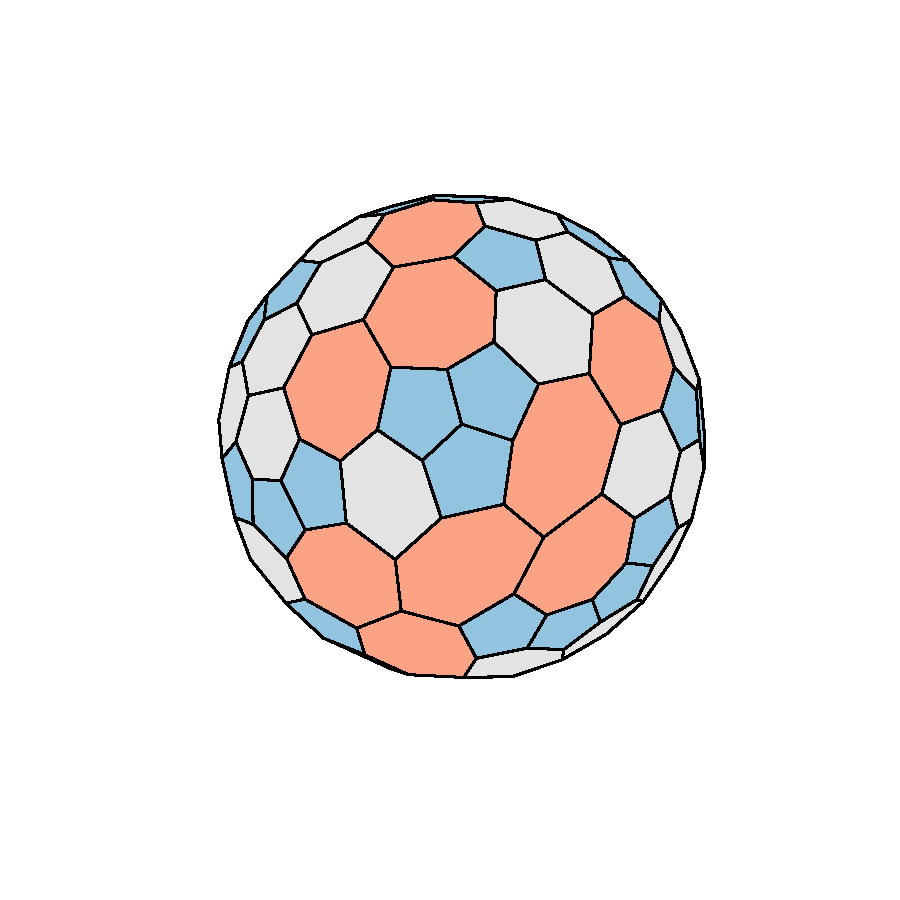
\includegraphics[width=\textwidth]{./figures/general_networks/full92_r-10.pdf}
         \caption{$p_6=36/92$,\\ $r=-0.1$}
         \label{fig:fullerene92b}
     \end{subfigure}
     \hfill
     \begin{subfigure}[b]{0.2\textwidth}
         \centering
         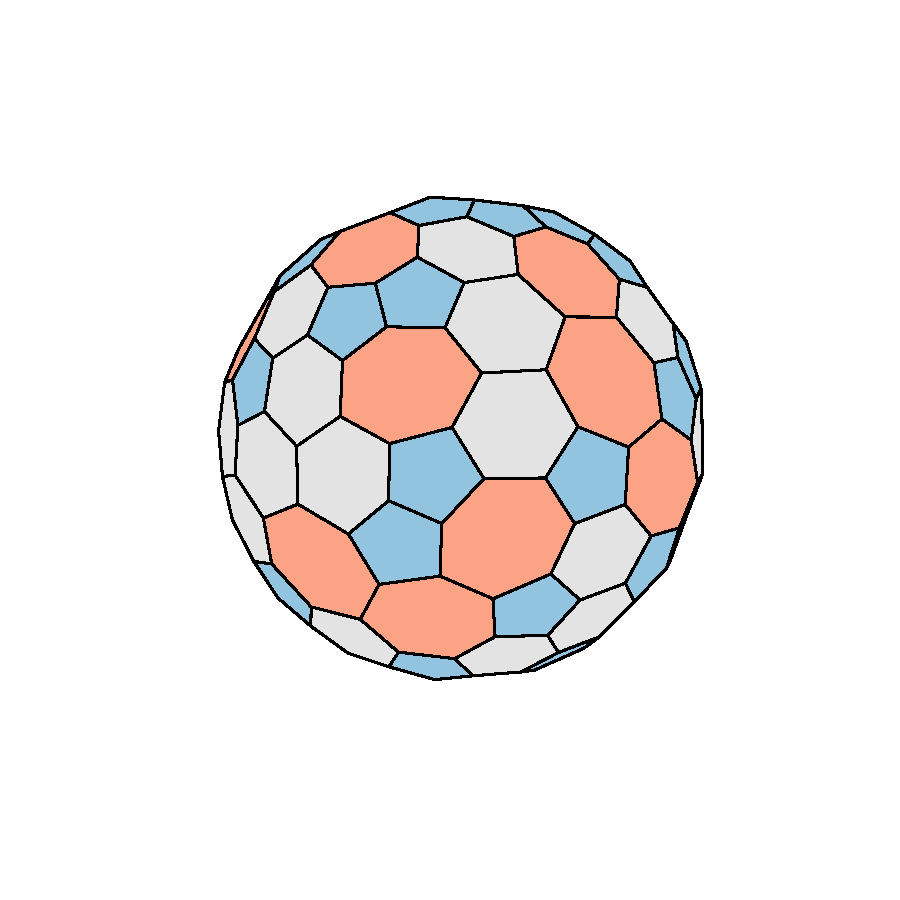
\includegraphics[width=\textwidth]{./figures/general_networks/full92_r-30.pdf}
         \caption{$p_6=36/92$,\\ $r=-0.3$}
         \label{fig:fullerene92c}
     \end{subfigure}
     \hfill
     
     \caption{Panel (a) gives a map of fullerene stability as a function of ring statistics and assortativity.
        Potential energy increases as more pentagons and heptagons are accommodated, but is also strongly related to their arrangement as shown by the value of the assortativity, $r$.
        Panels (b)-(d) give three example fullerenes with the same $p_6=36/92$ but different assortativities of $r=0.1,-0.1,-0.3$, respectively and as highlighted by the crosses in panel (a).}
     \label{fig:fullerene92}
\end{figure}

\section{Chapter Conclusions}

In summary, this chapter has thoroughly examined the network properties of a wide range of naturally occurring \td{} systems; spanning varying coordination environments, potential models and topologies.
Data has been collected from a range of experimental sources, and have the theoretical bond switching method has been further developed to aid the study of these diverse systems computationally.
These data have been analysed with rigorous metrics from network science, with the aim of highlighting the study of real\--world physical systems as an important and interesting addition to the wider field.
In particular these networks display unique constraints as a result of their underlying physics.
It has been shown that their mean node degree is fixed and the node degree distribution is well defined, following \lm's law.
In addition the concept of network assortativity has been introduced to measure ring correlations, and its preferability over the previous empirical measure known as the \aw{} law has been argued.
Although the assortativity has been shown to be a function of the potential model for a system and the limits of the assortativity linked to the occurrence of well\--known physical motifs; most physical networks show a very similar overall level of disassortativity, as experienced in nature.
An exception to this rule has also been found, where variable\--coordination systems can de\--mix to exhibit assortative behaviour.

In this chapter it has demonstrated how network science is applicable to understanding and analysing generic systems in physics, but also how physical systems form a key and under\--explored area of network science.
Going forward there is lots of potential scope to extend these explorations.
For example, there are still questions to be answered from this work such as how network properties such as the assortativity are explicitly related to the physics of the underlying system and whether this information can be utilised experimentally \-- for example to control and effectively quantify the pore size in materials.
This has also set up extensions to investigating more disordered networks still, such as biological networks which have a wider range of coordination environments.



 



